\documentclass[sigplan,10pt,review,anonymous]{acmart}

% Packages {{{
\usepackage{hyperref}
\usepackage{amsmath}
\usepackage{amssymb}
\usepackage{bbm}
\usepackage{tikz}
\usetikzlibrary{calc}
\usetikzlibrary{graphs}
\usetikzlibrary{cd}
\usepackage{bussproofs}
\usepackage{galois}
\usepackage{stmaryrd}
\usepackage{calc}
\usepackage{bbm}
\usepackage{soul}
\usepackage{booktabs}
% }}}

% Parameters {{{

\hyphenation{Comp-Cert}

% }}}

% Macros {{{

%\newtheorem{example}{Example}
%\newtheorem{definition}{Definition}
%\newtheorem{lemma}{Lemma}

\newcommand{\kw}[1]{\ensuremath{ \mathsf{#1} }}
\newcommand{\ifr}[1]{\mathrel{[{#1}]}}
\newcommand{\ifrw}[2]{\mathrel{[{#2} \Vdash {#1}]}}
\newcommand{\alt}{\ |\ } % use \mid instead
\newcommand{\bind}{\gg\!\!=}

\newcommand{\EC}{\kw{C}}
\newcommand{\simrel}{\kw{simrel}}

% Moves
\newcommand{\mcall}[3]{\kw{#1}({#2})@{#3}}
\newcommand{\pcall}[3]{%
  \underline{\mcall{#1}{#2}{#3}}%
}
\newcommand{\mret}[2]{{#1}@{#2}}
\newcommand{\pret}[2]{%
  \underline{\mret{#1}{#2}}%
}
\newcommand{\mretx}[3]{{#1}@{#2}/{#3}}
\newcommand{\pretx}[3]{%
  \underline{\mretx{#1}{#2}{#3}}%
}

% Pointers for justified sequences %{{{

% Parameters
\newcommand{\pshift}{1.6ex}
\newcommand{\pcdist}{2.5}
\newcommand{\pcangle}{60}

% Pointer hook
\newcommand{\ph}[1]{%
  \tikz[remember picture]{\coordinate (#1);}}

% Pointer to
\newcommand{\pt}[1]{%
  \rule{0pt}{1.4em}%
  \tikz[remember picture, overlay]{
    \draw[->]
      let \p{dest} = (#1),
          \n1 = {ln(veclen(\x{dest}, \y{dest}) + 1)},
          \p1 = ($(0,0)+(0,\pshift)$),
          \p4 = ($(#1)+(0,\pshift)$),
          \p2 = ($(\p1)!\n1*\pcdist!-\pcangle:(\p4)$),
          \p3 = ($(\p4)!\n1*\pcdist!+\pcangle:(\p1)$) in
        (\p1) .. controls (\p2) and (\p3) .. (\p4);}}

%}}}

% }}}

\title{Refinement-Based Game Semantics for CompCert}

\author{J\'er\'emie Koenig}
\affiliation{Yale University}
\email{jeremie.koenig@yale.edu}

\author{Zhong Shao}
\affiliation{Yale University}
\email{zhong.shao@yale.edu}

\begin{document}

\begin{abstract} %{{{
In recent years,
formal verification of computer systems
of increasing size has become practical.
Researchers have been able to verify complex artifacts
at a variety of abstraction levels spanning
from CPU designs to network protocols.
These achievements remain discrete efforts, but
there has been increasing interest in rendering them interoperable,
as exemplified by the DeepSpec project.
The ability to connect correctness proofs of components
verified at various levels of abstraction
would enable the construction of extremely reliable heterogenous systems
through end-to-end verification.

We propose that a successful synthesis of existing research on
game semantics,
refinement-based methods, and
abstraction layers
has the potential to serve as a common theory
of certified components.
We apply this methodology to define
a compositional semantics for the verified compiler
CompCert,
and to extend
the compiler's correctness proof
to the compositional setting
with much less effort than in previous attempts.
\end{abstract}
%}}}

\maketitle

\section{Introduction} %{{{

% preamble {{{

Over the past decade,
researchers have been able to formally verify the
total functional correctness
of various key components of computer systems,
including
compilers \cite{compcert, vellvm},
operating system kernels \cite{sel4, popl15},
file systems \cite{fscq}, and
processor designs \cite{safe}.
Such verification efforts
consist of
a formal semantics describing the system's behavior,
a formal specification,
and a mechanized proof that
the system conforms to the specification.
Assuming the semantic model and specification accurately describe
the system's operation and requirements,
this approach can provide
strong reliability guarantees.
Moreover,
if the proof is mechanized in a general-purpose proof assistant,
it can be validated by a third-party
without the need to trust the original developers.

%}}}

\subsection{Specifications as Interfaces} %{{{

Such achievements remain discrete efforts, but
there has been increasing interest in rendering them interoperable,
as exemplified by the DeepSpec project \cite{deepspec}.
By using formal specifications as interfaces
between the correctness proofs of various components ---
showing that the requirements of one component
are met by the guarantees of another ---
the researchers in DeepSpec hope to
verify composite systems
operating over a wide range of abstraction layers.
If successful,
this would represent a deployment of formal methods
at an unprecedented scale.

This methodology could also provide a qualitative increase
in the reliability of the resulting systems.
A certified component is only as trustworthy as its specification;
having specifications tied too much to a single verification effort
increases the risk of
implementation bugs being simply propagated to
the specification.
These bugs would become apparent in an effort to
connect the specification's guarantees to
the requirements of another component.
Moreover,
specifications used as internal interfaces
cease to be part of
the trusted base;
therefore,
building larger certified systems
by composing existing ones
reduces the
ratio between the size of the external specification to
the overall size of the system.

%}}}

\subsection{The CompCert C Compiler} %{{{

These principles are illustrated in
the certified C compiler CompCert \cite{compcert}.
The semantics of the various intermediate languages
used by CompCert are formalized as transition systems,
and the correctness of each pass is established
as a self-contained simulation between
the source and target programs for that pass.
As the various passes are composed into a complete compiler,
their correctness proofs are composed as well.
The final theorem no longer involves
intermediate languages,
but only the semantics of the source and target programs.

Since the introduction of CompCert a decade ago \cite{compcert},
there have been successful efforts aimed at
interfacing it with other verification tools \cite{vst},
using it as a component in larger verification projects \cite{popl15},
and refining its correctness theorem
to model real-world compiler use
in increasingly realistic detail
\cite{qompcert,sepcompcert,compcompcert,compcerttso,compcertshm}.
With each step,
the user can gain more confidence in the reliability of CompCert:
existing work testing the correctness of existing compilers
has found fewer bugs in CompCert,
compared to unverified alternatives \cite{csmith},
and efforts to make CompCert's correctness theorem more realistic
have uncovered and removed some of the few remaining bugs \cite{sepcompcert}.

%}}}

\subsection{Challenges} %{{{

However,
a long-standing limitation of CompCert is that
its language semantics
only model the operation of a complete program.
Previous attempts to extend them
to model the behavior of individual compilation units
\cite{compcompcert,cpp15}
have come at the cost of a significant increase
in the complexity of the proof,
preventing their adoption.
This limits the applicability of CompCert
to the construction of certified systems,
so that for instance in the work on CertiKOS \cite{popl15,osdi16,ccal},
adaptations have been necessary
to interface the compiler with the rest of the development.

More generally, many verification projects
use ad-hoc semantic models and specifications,
expressed in paradigms chosen first and foremost
to make modeling and verification tasks tractable.
Since verification is challenging,
the freedom to choose an appropriate semantic model
is quite valuable.
On the other hand,
the diversity of paradigms used for specification and verification
makes it difficult
to interface projects using different approaches.

These competing concerns
suggest the need to identify a common,
flexible semantic framework
into which existing models could be embedded
for integration purposes.
To enable building certified systems
from off-the-shelf components,
this framework should be equipped with
a rich composition infrastructure
and high-level principles for
reasoning about composite systems.
We propose that
a successful synthesis of existing research
on game semantics,
refinement-based verification,
and certified abstraction layers
could provide a general framework
for the construction of large-scale certified systems.
We call this approach \emph{refinement-based game semantics}.

%}}}

\subsection{Contributions} %{{{

In this paper,
we combine these ingredients into a single theory
and use it to construct a
compositional semantics for CompCert.
Our approach builds on previous attempts
but does not require significant changes
to CompCert's simulation relations and correctness proofs:
our framework is sufficiently expressive to
characterize them, and
sufficiently powerful to enable compositionality
by strengthening them
using properties of the languages involved.

%
%In \S\ref{sec:mainideas},
%we examine from a more formal perspective
%the principles enabling the construction
%of large-scale certified systems,
%and describe our high-level vision of
%refinement-based game semantics.
%In \S\ref{sec:monad},
%we construct a semantic framework, formalized in the Coq proof assistant,
%which augments a simple game model
%with abstraction and refinement.
%We demonstrate its applicability in \S\ref{sec:modsem}
%by using it to formulate a compositional module semantics
%for CompCert.
%In \S\ref{sec:compcert},
%we show that a high-level
%\emph{calling convention algebra}
%can be used to make the correctness theorem of CompCert
%fully compositional,
%with only minimal changes to the existing correctness proofs.

%}}}

%}}}

\section{Main Ideas} \label{sec:mainideas} %{{{

\subsection{Principles for system construction} %{{{

% preamble {{{

The goal of certified system design is
to create a formal description of
the system to be constructed (the program),
while ensuring through careful analysis that the system
will behave properly.
To carry out this analysis,
we must assign
to a system description $p \in P$
a mathematical object $\llbracket p \rrbracket \in \mathbb{D}$
representing its behavior.
We will call the set $\mathbb{D}$ a \emph{semantic domain}.
In this section we elucidate
the structure and properties of $\mathbb{D}$
necessary to the process of builing
large-scale certified systems.

%}}}

\subsubsection{Specifications and refinement} %{{{

System design starts with a set of requirements
that constrain the behavior of the system to be constructed
(the specification).
These requirements may not capture every detail
of the behavior of the eventual system,
but delineate a range of acceptable behaviors
from the point of view of its environment.

In refinement-based approaches,
programs and specifications are interpreted in the same
semantic domain $\mathbb{D}$,
which is equipped with a \emph{refinement} preorder
${\sqsubseteq} \subseteq \mathbb{D} \times \mathbb{D}$.
The proposition $\sigma_1 \sqsubseteq \sigma_2$
asserts that $\sigma_2$ is a refinement of $\sigma_1$,
and in particular a system description $p \in P$ is a correct implementation
of $\sigma \in \mathbb{D}$ when
$\sigma \sqsubseteq \llbracket p \rrbracket$.

%}}}

\subsubsection{Compositionality} %{{{

Complex systems are built by assembling components
whose behavior is understood,
such that their interaction achieves a desired effect.
The syntactic constructions of
the language used to describe systems
correspond to the ways in which they can be composed.

To enable compositional reasoning,
a suitable model must provide an account of
the behavior of the composite system
in terms of the behavior of its parts.
For instance,
if the language contains a binary operator
${+} : P \times P \rightarrow P$,
then the semantic domain should be equipped with
a corresponding operation
${\oplus} : \mathbb{D} \times \mathbb{D} \rightarrow \mathbb{D}$
such that:
$\llbracket p_1 + p_2 \rrbracket =
 \llbracket p_1 \rrbracket \oplus \llbracket p_2 \rrbracket$.

%}}}

\subsubsection{Monotonicity} %{{{

Once a component has been shown to conform to a given specification,
we want to abstract it as a ``black box''
so that further reasoning can be done in terms of
the component's specification rather than its implementation details.
To support this,
we must establish that semantic composition operators
are compatible with refinement:
\[ \sigma_1 \sqsubseteq \sigma_1' \wedge
   \sigma_2 \sqsubseteq \sigma_2' \Rightarrow
   \sigma_1 \oplus \sigma_2 \sqsubseteq \sigma_1' \oplus \sigma_2' \,. \]
Suppose we have two components $p_1$ and $p_2$,
where $p_2$ relies on $p_1$ for its operation,
and we want to verify that their combination $p_1 + p_2$
satisfies a specification $\sigma$.
Once we verify $p_1$ against its own specification
$\sigma_1 \sqsubseteq \llbracket p_1 \rrbracket$,
by the monotonicity of ${\oplus}$ means it is sufficient to show that
$\sigma \sqsubseteq \sigma_1 \oplus \llbracket p_2 \rrbracket$:
\[
   \sigma \:\sqsubseteq\:
   \sigma_1 \oplus \llbracket p_2 \rrbracket \:\sqsubseteq\:
   \llbracket p_1 \rrbracket \oplus \llbracket p_2 \rrbracket \:=\:
   \llbracket p_1 + p_2 \rrbracket
\]

%}}}

\subsubsection{Abstraction} %{{{

Large-scale systems operate across many layers of abstraction.
Each abstraction layer defines its own understanding of the interaction
between a component and its environment.
To relate abstraction layers we need to give
an explicit account of how their formulations of the interaction
correspond to one another.
In this work we address this by defining a heterogenous version
of the refinement relation
${\sqsubseteq_\mathbb{R}} \subset
 \mathbb{D}^\sharp \times \mathbb{D}^\natural$ between
the abstract domain $\mathbb{D}^\sharp$ and
the more concrete one $\mathbb{D}^\natural$, where 
$\mathbb{R}$ specifies a correspondance between
the two levels of abstraction
(a \emph{simulation convention}, see \S\ref{sec:modesem:sim}).

%In related work we show that for a sufficiently general
%semantic domain, the simulation convention $\mathbb{R}$
%defines a Galois connection
%$(\mathbb{D}^\sharp, {\sqsubseteq})
% \galois{\gamma}{\alpha}
% (\mathbb{D}^\natural, {\sqsubseteq})$
%between the abstract and concrete domains,
%which allows refinement properties to be transferred between
%the abstract and concrete domains through the defining property
%$
%    \gamma(\sigma^\sharp) \sqsubseteq \sigma^\natural \Leftrightarrow
%    \sigma^\sharp \sqsubseteq \alpha(\sigma^\natural)
%$.

%}}}

\subsubsection{Compilers} %{{{

This is particularly relevant
in the context of compilers.
Between C and assembly,
interactions across compilation units
are understood very differently.
At the level of C,
cross-module interaction is defined in terms of
function calls;
invoking a function consists of assigning values
to the function's parameters,
initializing a new stack frame,
and finally executing the function's body.
At the assembly level, cross-module
interactions simply consist in branching to an address
outside the current module with
a certain register state.

In that context,
the correpondance between the source and target semantic domains
depends on the \emph{calling convention} used by the compiler.
The correctness property of a C-to-assembly compiler
can then be stated as:
\[ \llbracket p \rrbracket_s \sqsubseteq_\mathbb{R}
   \llbracket C(p) \rrbracket_t \,. \]
where
$p$ is the source program, $C(p)$ the compiler's output,
$\llbracket - \rrbracket_s$ gives the semantics of the source language,
$\llbracket - \rrbracket_t$ gives the semantics of the target language,
and $\mathbb{R}$ formalizes the C calling convention.

%}}}

%}}}

\subsection{Game semantics} %{{{

% preamble {{{

Game semantics is a form of denotational semantics which
incorporates some operational aspects.
An early success of this approach was
the formulation of the first satisfactory, fully abstract models
of the programming language PCF \cite{pcfajm,pcfho}.
In this section,
we give an overview of this line of research
and how it can be applied in the context of CompCert.

Typically,
types are interpreted as two-player games,
which correspond to the interaction
between a program component of the given type
(the player \kw{P}, for \emph{proponent})
and its execution context
(the player \kw{O}, for \emph{opponent}).
The behavior of a term or component
is then modeled as a strategy for \kw{P} in this game,
which specifies the next move of the component
for all relevant positions in the game.

Positions are usually identified with sequences of moves,
and strategies can be identified with the set of positions
that a component can reach.
In this sense,
game semantics is similar to
the trace semantics of process algebras.
However, game semantics is distinguished
by a strong polarization between
the system and the environment,
and a strong distinction between outputs and inputs.
This confers an inherent ``rely-guarantee'' flavor
to games which facilitates compositional reasoning
in the context of heterogenous systems \cite{cspgs}.

%}}}

\subsubsection{Games} \label{sec:mainideas:gs:games} %{{{

A game is usually defined by giving a set of moves $M$
that players can choose from,
as well as a specification of which
sequences of moves are considered valid.
For chess,
moves will be taken in the set $(\{a, \ldots, h\} \times \{1, \ldots, 8\})^2$,
and a valid sequence of moves may look like:
\[ e2e4 \cdot \underline{c7c5} \cdot c2c3 \cdot \underline{d7d5} \cdots \]
As a more relevant example,
the game $\mathcal{C}$ is defined in \S\ref{sec:compcert:li}
to model the semantics of C compilation units,
It describes the behavior of a single function call,
so that its plays are of the form:
\[ f[sg](\vec{v})@m \cdot \underline{v'@m'} \]
The environment indicates
which function $f$ should be invoked
using what signature $sg$,
and specifies the values $\vec{v}$ of the arguments
as well as the state $m$ of the memory
at the time of invocation.
When the function returns,
the system replies with a move $v'@m'$,
transferring control back to the environment
with the return value $v'$
and the updated memory state $m'$.
For simplicity,
we will omit signatures and memory states
from examples given in this section.

We will focus on two-player, alternating games
where the environment and the system each contribute every other move.
The environment plays first.
When typesetting examples,
we underline the moves of the second player
(the system).

Most game semantics
include additional structure
in the description of games.
The set of moves is usually partitioned
into proponent and opponent moves ($M = M^\kw{O} \uplus M^\kw{P}$),
and into questions and answers ($M = M^\kw{Q} \uplus M^\kw{A}$).
Game models for high-order languages are often more complex.

%}}}

\subsubsection{Strategies} \label{sec:mainideas:gs:strat} %{{{

Following trace semantics of process calculi,
traditional work on game semantics
represents strategies as
the set of positions that the player may reach.
Hence,
a strategy is a prefix-closed set of finite sequences of moves.
For example,
the strategy $\sigma$ used by
the black player in the chess play above
contained the plays:
\[
  \sigma \: = \: \{
    e2e4, \quad
    e2e4 \cdot \underline{c7c5}, \quad
    e2e4 \cdot \underline{c7c5} \cdot c2c3, \quad
    \ldots
  \}
\]

Strategies are usually subject to a number
of well-formedness constraints beyond prefix closure.
Commonly used contraints include the following \cite{gamesem99}:
\begin{description}
\item[Receptivity]
  requires that all possible behaviors of the environment
  be included in the strategy,
  so that if $s \in \sigma$ is an even-length play and
  $m$ is an environment move such that $sm$ is a valid play of the game,
  then $sm \in \sigma$ as well.
\item[Determinism]
  prevents the strategy from allowing
  more than one observable behavior of the system at any given point,
  so that if $s \in \sigma$ is an odd-length play,
  then any moves $m, n$ of the system
  such that $sm \in \sigma$ and $sn \in \sigma$
  must be equal ($m = n$).
\item[Well-bracketing]
  only allows the most recently asked question
  to be answered at any given point.
  That is,
  the game proceeds according to a strict stack discipline.
\item[Innocence]
  requires that the behavior of a strategy
  only depends on the most recent move
  as well as the chain of moves enabling it.
  This means the strategy is not allowed to maintain
  unobservable private state across
  successive but independent queries.
\end{description}
The game semantics of PCF
imposed all of these constraints,
and subsequent work was able to model additional language features
by relaxing combinations of them.
%Following \cite{gsnondet},
%we will relax the determinism constraint in order
%to model specifications permitting
%a range of implementation behaviors.
The family of games we consider,
and the representation we use for strategies,
are restrictive enough that
the well-bracketing and innocence constraints
will always be satisfied.

%}}}

\subsubsection{Compositionality} \label{sec:mainideas:gs:comp} %{{{

While the game $\mathcal{C}$
presented in \S\ref{sec:mainideas:gs:games}
is extremely simple,
the expressive power of game semantics
comes from the way in which complex games can be derived from simple ones,
and used to interpret compound types.
In the following we recall common constructions
and demonstrate their use
in our semantic model for C compilation units.

For a game $E$,
the game $!E$ consists of multiple copies of $E$,
instantiated at the discretion of the environment.
For example,
the following is a play for the game $!\mathcal{C}$:
\[
    \kw{pow}(3,2) \cdot
    \underline{9} \cdot
    \kw{pi}() \cdot
    \underline{3.1416} \cdot
    \kw{pow}(5,0) \cdot
    \underline{1}
\]
Because $\mathcal{C}$ has a very simple structure
and our strategies are alternating,
in this example the different copies of $\mathcal{C}$
will always be played in succession.
However,
in richer models multiple copies may proceed
concurrently
and be played in an interleaved manner.

Another common construction is the game $E \multimap F$
in which $E$ and $F$ are played side-by-side.
In the game $E$ the roles of the system and the environment
are reversed.
In our context,
the game will always start
with a move of $F$ played by the environment,
but the system may subsequently initiate the game $E$.
For instance, a strategy $\sigma$
for the game $\mathcal{C} \multimap \mathcal{C}$
may include plays of the form:
\[
    \sigma \: \ni \:
    \kw{pow}(3,2) \cdot
    \underline{\kw{mult}(3,3)} \cdot
    r \cdot
    \underline{r}
\]
Here,
the component's function $\kw{pow}$
is invoked (in the right-hand side game),
but instead of immediately returning a result,
the component performs an external call to $\kw{mult}$.
After the environment replies with the result $r$,
the component answers the invocation of $\kw{pow}$
with the same value.

Two strategies
$\phi : A \multimap B$ and
$\gamma : B \multimap C$ can be composed
to yield a strategy $\gamma \circ \phi : A \multimap C$
which behaves like $\gamma$,
but uses $\phi$ to fulfill any request made by $\gamma$
in the middle game $B$.
Any request of $\phi$ will in turn appear as
an external request of the composite strategy $\gamma \circ \phi$.
To build on our example,
if a component implements $\kw{mult}$
with the strategy:
\[ \rho := \{ \kw{mult}(n,p) \cdot \underline{r} \mid r = n p \} \,, \]
then the composition of $\sigma$ and $\rho$ will include the play:
\[ \sigma \circ \rho \ni \kw{pow}(3,2) \cdot \underline{9} \]

The constructions presented above can be used together
to express the structure of various kinds of interactions.
The type $!A \multimap B$ is traditionally used
to model the behavior of a $\lambda$-term of type $A \rightarrow B$,
which can access its argument multiple times.
In our context,
the game $\mathcal{C} \rightarrow \mathcal{C}$
represents the way a C compilation unit behaves in response to
an activation,
with the ability to perform any number of external calls.

%}}}

%}}}

%\subsection{Refinement} \label{sec:mainideas:gs:ref} %{{{
%
%Existing work on denotational game semantics of
%typed functional languages
%has not placed much emphasis on the notion of refinement,
%focusing instead on program equivalence and
%the problem of full abstraction.
%While there have been attempts to integrate nondeterminism
%to game semantics \cite{gsnondet,gsndsheaves},
%we believe that this work
%is limited by a lack of distinction between angelic and demonic
%nondeterminism.
%
%The distinction between system and environment actions
%present in game-theoretical approaches
%leads to a notion of \emph{alternating} refinement:
%a behavior $x$ refines a behavior $y$ if
%all \emph{system} actions in $x$ are also possible in $y$, and if
%all \emph{environment} actions in $y$ are also possible in $x$
%\cite{altref,gmos}.
%This makes it possible for specifications to
%constrain the environment as well as the system,
%and enables a rely-guarantee style of reasoning.
%
%In the realm of imperative program semantics and verification,
%it has long been recognized that predicate transformers
%can model both \emph{angelic} and \emph{demonic} nondeterminism,
%and that this duality has important connections to games.
%In particular,
%the imperative programs and specifications
%of the \emph{refinement calculus} are understood as
%\emph{contracts} between a component and its environment,
%and their behavior is described in terms of
%an operational game semantics \cite{refcal,refcalgames}.
%The calculus incorporates both kinds of nondeterminism
%as the meet and join operations of the calculus' refinement lattice.
%
%We build on recent work extending this approach to the realm
%of functional programming \cite{augtyp,dndf}
%to incorporate dual nondeterminism to the game semantics
%we present in \S\ref{sec:gamesem}.
%
%%}}}

\subsection{CompCert Semantics} %{{{

\begin{figure} % fig:compcerts {{{
  \begin{tabular}{lr}
    \hline
    Variant & Semantic model \\
    \hline
    CompCert \cite{compcert}, SepCompCert \cite{sepcompcert} &
      $\epsilon : \mathcal{E} \rightarrow \mathcal{C} \vdash
       \mathcal{E} \rightarrow \mathcal{N}$ \\
    CompCertX/CertiKOS \cite{popl15} &
      $\epsilon : \mathcal{E} \rightarrow \mathcal{C} \vdash
       \mathcal{E} \rightarrow \mathcal{C}$ \\
    Compositional CompCert \cite{compcompcert} &
      $\mathcal{C} \rightarrow \mathcal{C}$ \\
    Ramananandro et al. \cite{cpp15} &
      $\mathcal{E} \times \mathcal{C} \rightarrow \mathcal{C}$ \\
    This work &
      $\mathcal{E} \times E \rightarrow F$ \\
    \hline
  \end{tabular}
  \caption{Taxonomy of CompCert extensions in terms of games.}
  \label{fig:compcerts}
\end{figure}
%}}}

The conceptual framework of game semantics
can be used to classify previous work
on extending the semantic model of CompCert.
Figure~\ref{fig:compcerts}
enumerates the semantic models
used by several variants of CompCert
and the type of strategies they encode.

Components listed on the left of the turnstile ($\vdash$)
represent static, global parameters of the semantics,
whereas games which appear on the left of $\rightarrow$
describe a dynamic interaction
encoded by the corresponding semantic objects.

\subsubsection{Whole-program semantics} %{{{

In the original CompCert,
programs are invoked without any parameters
and they produce a single machine integer denoting their exit status.
This can be described by the game $\mathcal{N}$,
whose plays are of the form ${*} \cdot \underline{n}$,
with $n \in \mathbb{B}^{32}$.

During their execution,
their interaction with the environment
is captured as a trace of events from a limited set,
each event having an output and input component ($\mathcal{E}$).

CompCert accounts for external calls
in a limited way:
the entire semantics is parametrized by
the behavior $\epsilon$ of external functions.
The correctness proof assumes that $\epsilon$ is deterministic
and that it satisfies a number of healthiness requirements
with respect to the memory transformations
used in CompCert's correctness proof.

%}}}

\subsubsection{Contextual compilation} %{{{

This is generalized slightly in CompCertX \cite{popl15},
where program invocations specify
the function to be called,
values for its arguments,
as well as the initial state of the memory,
and terminations carry
the function's return value and final memory state
($\mathcal{C}$).
This allows CompCertX and its correctness theorem
to be used in the layer-based verification of
the operating system kernel CertiKOS:
once CompCertX has been used to
analyze and verify the code of a given abstraction layer,
that code can be used as the new $\epsilon$
when a higher-level module is verified in turn.
This enabled the verification of CertiKOS ---
an artifact of significant size ---
at the level of assembly code,
by integrating CompCert as part of its proof of correctness.
However,
this approach does not support two-way invocations between components,
and in addition
it requres the healthiness requirements on $\epsilon$
to be esablished before
more code can be built on top of it.

%}}}

\subsubsection{Compositional compilation} %{{{

A more comprehensive form of compositionality
is provided by
the semantic model of \cite{cpp15},
and especially by
the work on Compositional CompCert \cite{compcompcert}.
In the former,
the existing event trace infrastructure of CompCert
is augmented to include external calls as a type of events.
In Compositional CompCert,
the labelled transition systems and the associated
event trace infrastructure are replaced by
\emph{interaction semantics}.
Interaction semantics is a form of operational game semantics.
The interactions between a component and its environment
are identified by additional predicates on program states and
captured in terms of C function calls as previously described.

Beyond this technical difference,
the two approaches are distinguished by
how they handle refinement.
The function calls and returns described by $\mathcal{C}$
include memory states,
which are not identically preserved by compilation;
this makes it difficult to directly compare the behaviors
of the source and target programs.
In \cite{cpp15},
this is handled by strengthening the memory transformations
used by the compiler into bijective mappings;
such mappings can then be applied to the entire execution trace
to establish refinement.
However, several passes of CompCert are challenging
to fit into this framework.
By contrast,
Compositional CompCert
embraces a more general relational approach,
with a clear distinction between the role of the system
and that of the environment:
given executions of the source and target programs,
the system guarantees that outputs are related
under the assumption that the environment has provided related inputs.

%}}}

\subsubsection{Typed components} %{{{

Our approach is closest to that of Compositional CompCert,
however we extend the model in several important ways.
In particular,
while interaction semantics
only accounts for interactions of the form
described above as the game $\mathcal{C}$,
we generalize this to a typed setting,
where the types of incoming and outgoing calls and returns
are specified by an \emph{elementary game}
with a similarly simple structure;
therefore,
a transition system $L$ is assigned a type $L : E \rightarrow F$,
where $E, F$ are elementary games.
We define and choose suitable games
for all intermediate languages,
as summarized in Table~\ref{tbl:li}.
The semantics of the source language Clight
is expressed in terms of the game $\mathcal{C} \rightarrow \mathcal{C}$,
whereas the semantics of the target language Asm
is expressed in terms of the game $\mathcal{A} \rightarrow \mathcal{A}$.
This means we can accurately model assembly-level control transfers.
This is crucial when verifying system code
which incorporates hand-written assembly components
which do not follow the C calling convention.

Embracing the difference between the interfaces of
the source and target languages
represents a significant departure from established practice.
Existing work goes great lengths
to ensure that the source and target semantics
are expressed in the same semantic domain.
Indeed,
the success of CompCert itself
relies in part on its use of a flexible
but uniform memory model,
capable both of modeling the C standard accurately,
and of giving a reasonable account
of assembly-level mechanics.
Later work such as \cite{compcompcert,cpp15}
follows this precedent and uses
a uniform interface for open modules,
and treats source and target calls
as essentially the same,
and ensuring that any differences introduced by the compiler
are absorbed by a semantic framework
defined \emph{modulo} memory transformations.

By breaking with this approach,
we are led to introduce a notion of \emph{simulation convention},
which generalizes the usual concept of calling convention
and expresses the correspondance between
source- and target-level interactions.
This gain in expressivity
allows us to side-step a number of issues
that have plagued previous work on CompCert compositionality.

%}}}

\subsubsection{Simulations} %{{{

A simulation convention $\mathbb{R} : E_1 \Leftrightarrow E_2$
expresses the correspondance between
the source-level elementary game $E_1$ and
the target-level elementary game $E_2$.
Hence,
a simulation between
a source-level transition system $L_1 : E_1 \rightarrow F_1$ and
a target-level transition system $L_2 : E_2 \rightarrow F_2$ 
is assigned a type $\mathbb{R}_E \rightarrow \mathbb{R}_F$,
where
$\mathbb{R}_E : E_1 \Leftrightarrow E_2$ and
$\mathbb{R}_F : F_1 \Leftrightarrow F_2$.
We write:
\[
  L_1 \le_{\mathbb{R}_E \rightarrow \mathbb{R}_F} L_2 \qquad
  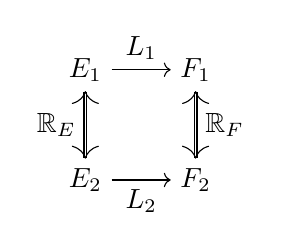
\begin{tikzpicture}[baseline,scale=0.7]
    \node (A1) at (-1,  1) {$E_1$};
    \node (A2) at (-1, -1) {$E_2$};
    \node (B1) at ( 1,  1) {$F_1$};
    \node (B2) at ( 1, -1) {$F_2$};
    \draw (A1) edge[->] node[auto] {$L_1$} (B1);
    \draw (A2) edge[->] node[auto,swap] {$L_2$} (B2);
    \draw (A1) edge[<->, double] node[auto,swap] {$\mathbb{R}_E$} (A2);
    \draw (B1) edge[<->, double] node[auto] {$\mathbb{R}_F$} (B2);
  \end{tikzpicture}
\]

Simulations compose as expected:
given the simulation conventions
$\mathbb{R} : E_1 \Leftrightarrow E_2$ and
$\mathbb{S} : E_2 \Leftrightarrow E_3$,
the composite convention
$\mathbb{R} \circ \mathbb{S} : E_1 \Leftrightarrow E_3$
describes the type composite simulations:
\[
  \AxiomC{$L_1 \le_{\mathbb{R}_E \rightarrow \mathbb{R}_F} L_2$}
  \AxiomC{$L_2 \le_{\mathbb{S}_E \rightarrow \mathbb{S}_F} L_3$}
  \BinaryInfC{$L_1 \le_{\mathbb{R}_E \circ \mathbb{S}_E \rightarrow \mathbb{R}_F \circ \mathbb{S}_F} L_3$}
  \DisplayProof
  \qquad
  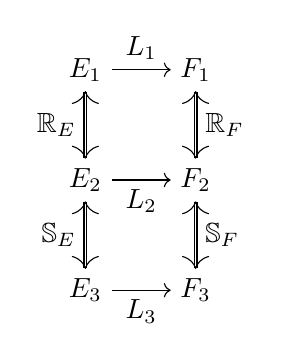
\begin{tikzpicture}[baseline,scale=0.7]
    \node (A1) at (-1,  2) {$E_1$};
    \node (A2) at (-1,  0) {$E_2$};
    \node (A3) at (-1, -2) {$E_3$};
    \node (B1) at ( 1,  2) {$F_1$};
    \node (B2) at ( 1,  0) {$F_2$};
    \node (B3) at ( 1, -2) {$F_3$};
    \draw (A1) edge[->] node[auto] {$L_1$} (B1);
    \draw (A2) edge[->] node[auto,swap] {$L_2$} (B2);
    \draw (A3) edge[->] node[auto,swap] {$L_3$} (B3);
    \draw (A1) edge[<->, double] node[auto,swap] {$\mathbb{R}_E$} (A2);
    \draw (B1) edge[<->, double] node[auto] {$\mathbb{R}_F$} (B2);
    \draw (A2) edge[<->, double] node[auto,swap] {$\mathbb{S}_E$} (A3);
    \draw (B2) edge[<->, double] node[auto] {$\mathbb{S}_F$} (B3);
  \end{tikzpicture}
\]
In addition,
simulation conventions of a given type
are equipped with a notion of refinement $\preceq$,
and for ``endo-conventions'' of type $\mathbb{R} : E \Leftrightarrow E$,
a corresponding notion of Kleene star $\mathbb{R}^*$.

%}}}

\subsubsection{Compiler Correctness} \label{sec:compcert:overview} %{{{

The semantics of CompCert $\kw{Clight}$ and $\kw{Asm}$ programs
can be expressed as interactive behaviors of types:
\[
    \kw{Clight} \llbracket p_s \rrbracket :
      \mathcal{C} \rightarrow \mathcal{C} \,, \qquad
    \kw{Asm} \llbracket p_t \rrbracket :
      \mathcal{A} \rightarrow \mathcal{A} \,.
\]
We will show that there exists a simulation convention
$\mathbb{R}_\kw{CompCert} : \mathcal{A} \Leftrightarrow \mathcal{C}$
such that whenever $p_t = \kw{CompCert}(p_s)$,
the following refinement property holds:
\begin{equation}
    \label{eqn:correctness}
    \kw{Asm} \llbracket p_t \rrbracket \,
    \le_{\mathbb{R}_\kw{CompCert} \rightarrow \mathbb{R}_\kw{CompCert}}
    \kw{Clight} \llbracket p_s \rrbracket
\end{equation}

In Compositional CompCert,
this is achieved independently for each compilation pass.
Stated in our terms,
Compositional CompCert
employs a fixed interface $\mathcal{C}$,
and \emph{structured injections} define a refinement convention
$\mathbb{S} : \mathcal{C} \Leftrightarrow \mathcal{C}$.
A theorem similar to (\ref{eqn:correctness}) is proved for each pass,
and structured injections are shown to compose
($\mathbb{S} \cdot \mathbb{S} \equiv \mathbb{S}$),
so that a theorem can be derived for the whole compiler.

%A major challenge encountered in this context
%is the asymmetry of requirements vs. guarantees
%present in the existing proofs:
%while CompCert imposes strong requirements
%on the semantics of external functions,
%the simulation relations used by its correctness proofs
%are too weak to establish corresponding guarantees
%for a module's own function executions,
%preventing horizontal compositionality.
%Because of this,
%Compositional CompCert required significant changes
%to all compilation passes,
%strengthening their simulation relations
%to conform to $\mathbb{S}$.

Our explicit treatment of abstraction
and reified notion of simulation convention
makes another approach possible.
Existing proofs can be adapted to establish
for each pass:
\begin{equation}
    \label{correctness-alt}
    \llbracket p_t \rrbracket
    \le_{\mathbb{R} \rightarrow \mathbb{R}'}
    \llbracket p_s \rrbracket \,,
\end{equation}
where the simulation conventions $\mathbb{R}$ and $\mathbb{R}'$
characterize the assumptions and guarantees of the proof.
In addition,
relevant properties of key source, target, and intermediate languages
can be expressed in relational form,
and can be used to strengthen the resulting theorem:
by composing these proofs together,
and using algebraic properties of
the simulation conventions involved,
we are able to bridge the gap
between the domain and codomain simulation conventions
and prove a correctness statement
in the form of (\ref{eqn:correctness}),
enabling horizontal compositionality.

%}}}

%}}}

\subsection{Logical relations} %{{{

Logical relations are structure-preserving relations,
in the same way that homomorphisms are structure-preserving maps.
However,
logical relations are more compositional than homomorphisms,
because they do not suffer from the same problems
in the presence of mixed-variance constructions,
such as the function arrow $\rightarrow$ \cite{lrp}.
In the context of typed languages,
this means type-indexed logical relations
can be defined by recursion over the structure of types.

%Logical relations have found widespread use in programming language theory.
%Unary logical relations can be used to establish
%various properties of type systems:
%a type-indexed predicate expressing a property of interest
%is shown to be compatible with the language's reduction,
%and to contain all of the well-typed terms of the language.
%Binary logical relations can be used to capture
%contextual equivalence between terms,
%as well as notions such as non-interference or compiler correctness.
%Relational models of type quantification yield
%Reynold's well-known theory of relational parametricity,
%and can be used to prove \emph{free theorems} that
%all terms of a given parametric type must satisfy.

Logical relations can be of any arity,
but in the present work
we will restrict our attention to
binary logical relations.
Given an algebraic structure $\mathcal{S}$,
a \emph{logical relation}
between two instances $S_1, S_2$ of $\mathcal{S}$
will be a relation $R$
between their carrier sets,
such that the corresponding operations of $S_1$ and $S_2$
take related arguments to related results.
We write $R : \mathcal{R}(S_1, S_2)$.

\begin{example}[Logical relation of monoids]
\label{ex:monoid}
A \emph{monoid} is a set $A$ equipped with
an associative binary operation $\cdot$ and
an identity element $\epsilon$.
A \emph{logical relation of monoids} between
a monoid $\langle A, \cdot_A, \epsilon_A \rangle$ and
a monoid $\langle B, \cdot_B, \epsilon_B \rangle$
is a relation $R \subseteq A \times B$
such that:
\[
(u \ifr{R} u' \wedge v \ifr{R} v' \Rightarrow u \cdot_A v \ifr{R} u' \cdot_B
v')
\: \wedge \:
\epsilon_A \ifr{R} \epsilon_B \,.
\]
\end{example}

Logical relations between multisorted structures
will include one relation for each sort,
between the corresponding carrier sets.
In the case of structures which include type operators,
we can associate to each base type $A$
a relation over its carrier set $\llbracket A \rrbracket$,
and to each type operator $T(A_1, \ldots, A_n)$
a corresponding \emph{relator}:
given relations $R_1, \ldots, R_n$ over
the carrier sets $\llbracket A_1 \rrbracket, \ldots, \llbracket A_n \rrbracket$,
the relator for $T$
will construct a relation $T(R_1, \ldots, R_n)$
over $\llbracket T(A_1, \ldots, A_n) \rrbracket$.

\begin{figure} % fig:relators {{{
  {\small
  \begin{align*}
    x \ifr{R_1 \times R_2} y \ \Leftrightarrow\  &
      \pi_1(x) \ifr{R_1} \pi_1(y) \wedge
      \pi_2(x) \ifr{R_2} \pi_2(y) \\
    x \ifr{R_1 + R_2} y \ \Leftrightarrow\  &
      (\exists \, x_1 \, y_1 \,.\,
        x_1 \ifr{R_1} y_1 \wedge
        x = i_1(x_1) \wedge
        y = i_1(y_1)) \\ \vee\ &
      (\exists \, x_2 \, y_2 \,.\,
        x_2 \ifr{R_2} y_2 \wedge
        x = i_2(x_2) \wedge
        y = i_2(y_2)) \\
    f \ifr{R_1 \rightarrow R_2} g \ \Leftrightarrow\  &
      \forall \, x \, y \,.\,
        x \ifr{R_1} y \Rightarrow
        f(x) \ifr{R_2} g(y) \\
    A \ifr{\mathcal{P}^\le(R)} B \ \Leftrightarrow\  &
      \forall \, x \in A \,.\,
      \exists \, y \in B \,.\,
      x \ifr{R} y
  \end{align*}
  }%
  \caption{A selection of relators}
  \label{fig:relators}
\end{figure}
%}}}

Relators for some common constructions are shown in Fig.~\ref{fig:relators}.
Note that the first requirement given in Example~\ref{ex:monoid} above
can be expressed as
$
  \cdot_A \ifr{R \times R \rightarrow R} \cdot_B
$.

%Logical relations used to reason about contextual equivalence
%are often partial equivalence relations (PER).
%By contrast, since we mainly focus on refinement,
%most of the relations we consider will not be symmetric.

%}}}

\subsection{Kripke logical relations} %{{{
\label{sec:klr}

For stateful languages,
which terms should be related
will often depend on the current state.
Kripke logical relations
are parametrized over a set of state-dependent \emph{worlds}.
Different components related at the same world
will be guaranteed to be related in compatible ways.

In the following,
we give a general account of Kripke logical relations
by drawing on their connection with
the Kripke semantics of modal logic.
We apply this framework
in our treatment of refinement and abstraction
in the context of game semantics (\S\ref{sec:monad:abs}).
Then in \S\ref{sec:compcert:cklr},
we use it to develop a logical-relations
understanding of some key aspects of CompCert,
and show how parametricity
can be used to derive important properties
of CompCert languages.

\begin{definition}
For a set $W$,
a \emph{Kripke logical relation} is
a family of logical relations $(R_w)_{w \in W}$.
We write $R : \mathcal{R}_W(S_1, S_2)$
for a Kripke logical relation between structures $S_1$ and $S_2$,
and define:
\begin{align*}
  x \ifr{w \Vdash R} y &\Leftrightarrow x \ifr{R_w} y \\
  x \ifr{\Vdash R} y &\Leftrightarrow \forall w \,.\, x \ifr{R_w} y \,.
\end{align*}
\end{definition}

\begin{example}[CompCert memory injections] \label{ex:meminj} %{{{
The memory model of CompCert divides the memory into blocks,
whose contents are addressed by an integer
(see \S\ref{sec:sem:mm}).
Between the states of the source and target programs,
a block may be dropped, added, or
mapped at a given offset within a larger block.
These transformations of the memory structure
are specified by partial functions of type:
\[
  \kw{meminj} := \kw{block} \rightharpoonup \kw{block} \times \mathbb{Z} \,,
\]
The simulation relations of CompCert,
and the component relations that they are built from,
are often parametrized by such a partial function $f : \kw{meminj}$,
which we call an \emph{injection mapping}.
An entry $f(b) = (b', o)$
means that the source memory block with identifier $b$
is mapped into the target memory block with identifier $b'$
at offset $o$.

For example,
CompCert represents pointers as pairs $(b, o)$, where
$b : \kw{block}$ designates a memory block, and
$o : \mathbb{Z}$ specifies an offset within the block.
The correspondance between source and target pointers
depends on the injection mapping being used.
To make sure pointers are related consistently
with each other and with the memory states,
in \S\ref{sec:compcert:mm}
we model this correspondance as a $\kw{meminj}$-indexed
Kripke logical relation $(R^\kw{ptr}_f)_{f : \kw{meminj}}$
defined by:
\[
    (b_1, o_1) \ifr{f \Vdash R^\kw{ptr}} (b_2, o_2) \:\Leftrightarrow\:
    f(b_1) = (b_2, o_2 - o_1) \,.
\]
\end{example}
%}}}

\subsubsection{Kripke relators}

A logical relation $R : \mathcal{R}(A, B)$
can be promoted to a $W$-indexed Kripke logical relation $\lceil R \rceil$
which ignores the index, so that $\lceil R \rceil_w = R$ for all $w \in W$.
Likewise,
a relator
  $F : \mathcal{R}(A_1, B_1) \,\times\,\cdots\,\times\,\mathcal{R}(A_n, B_n) \rightarrow \mathcal{R}(A, B)$
can be promoted to its Kripke version
by pointwise extension over the set of possible worlds:
\begin{gather*}
  \lceil F \rceil : \mathcal{R}_W(A_1, B_1) \times \cdots \times \mathcal{R}_W(A_n, B_n) \rightarrow \mathcal{R}_W(A, B) \\
  \lceil F \rceil (R_1, \ldots, R_n)_w = F(R_{1,w}, \ldots, R_{n,w})
\end{gather*}
We use $\lceil - \rceil$ implicitly
when a relator appears in a context where
a Kripke logical relation is expected.

\subsubsection{Modalities}

Kripke logical relations
can be used to ensure that the components of complex states
are related consistently (at the same world).
By adding structure to the set of worlds,
we will be able to go one step further and
specify how these worlds can evolve,
for instance across time.

\begin{definition} %{{{
A \emph{Kripke frame} is a tuple
$\langle W, {\leadsto} \rangle$, where
$W$ is a set of \emph{possible worlds} and
$\leadsto$ is a
binary \emph{accessibility relation} over $W$.
For a frame
$\langle W, \leadsto \rangle$,
we define the Kripke relators $\Diamond$, $\Box$ as:
\begin{align*}
  x \ifr{w \Vdash \Diamond R} y & \: \Leftrightarrow \:
    \exists \, w' \,.\, w \leadsto w' \wedge
      x \ifr{w' \Vdash R} y \\
  x \ifr{w \Vdash \Box R} y & \: \Leftrightarrow \:
    \forall \, w' \,.\, w \leadsto w' \Rightarrow
      x \ifr{w' \Vdash R} y
\end{align*}
\end{definition}
%}}}

Building on Example~\ref{ex:meminj},
we continue to examine the ways in which
some aspects of CompCert can be understood
in terms of Kripke logical relations.

\begin{example}[CompCert simulation diagrams] \label{ex:sim} %{{{
Many simulation diagrams in CompCert
involve a memory injection.
We can make them more compositional by
expressing them in the framework of Kripke logical relations.
A simulation relation will be a Kripke logical relation
$R \in \mathcal{R}_\kw{meminj}(A, B)$,
which will relate two transition systems
$\alpha : A \rightarrow \mathcal{P}(A)$ and
$\beta : B \rightarrow \mathcal{P}(B)$
according to the diagram:
\[
  \begin{tikzcd}
    s_1 \arrow[r, "\alpha"]
        \arrow[d, dash, "R_f"'] &
    s_1' \arrow[d, dashed, dash, "R_{f'} \quad (f \subseteq f')"] \\
    s_2 \arrow[r, dashed, "\beta"] &
    s_2'
  \end{tikzcd}
\]
More precisely, this diagram represents the following condition:
\begin{equation}
    \label{eqn:hairy-sim}
    \forall f \, s_1 \, s_2 \, s_1' \,.\,
      s_1 \ifr{f \Vdash R} s_2 \wedge
      \alpha(s_1) \ni s_1' \Rightarrow
    \exists f' \, s_2' \,.\,
      \beta(s_2) \ni s_2' \wedge
      f \subseteq f' \wedge
      s_1' \ifr{f' \Vdash R} s_2'
\end{equation}
Here, the new states may be related according to
a new memory injection $f'$,
but in order to preserve existing relationships
between source and target pointers,
the new memory injection should include
the original one ($f \subseteq f'$).

This pattern is very common in CompCert
and appears in a variety of contexts.
By using $\langle \kw{meminj}, {\subseteq} \rangle$
as a Kripke frame,
we can express it concisely and compositionally
in our relational framework.
For instance,
using the relator $\mathcal{P}^\le$ defined in
Fig.~\ref{fig:relators},
the condition (\ref{eqn:hairy-sim}) above can be expressed
concisely and legibly as:
\[
  \alpha \ifr{\Vdash R \rightarrow \mathcal{P}^\le(\Diamond R)} \beta \,.
\]
\end{example}
%}}}

%}}}

%}}}

\section{Operational Semantics} \label{sec:compcert} %{{{

This section describes the semantic model used by CompCertO.
First, in \S\S\ref{sec:sem:mm}--\ref{sec:sem:closed},
we review the techniques used in CompCert
to formalize the semantics of the various languages involved:
they are defined using labelled transition systems
operating over states are constructed around
a common memory model.
Then starting with \S\ref{sec:sem:li},
we describe our extensions to these techniques
to account for \emph{open modules}
and model the building process more closely.

\subsection{Introduction} \label{sec:sem:intro} %{{{

The semantics of CompCert languages
are constructed around a simple notion of process behavior.
By \emph{process}, we mean a self-contained computation
which can be characterized by
the possible sequences of system calls it performs.
Several steps are involved to go
from a source program to an executing process;
these steps are modeled by CompCert
with varying degrees of sophistication and accuracy.

In practice,
for a C program to be executed,
its translation units must first be compiled to object code.
Then,
the compiled object files must be linked together
into an executable binary file.
Finally, the system loads the binary into memory,
and some bootstrap runtime code
is used to set up the process state
and invoke to program's \kw{main} function.

\begin{figure} % fig:process {{{
    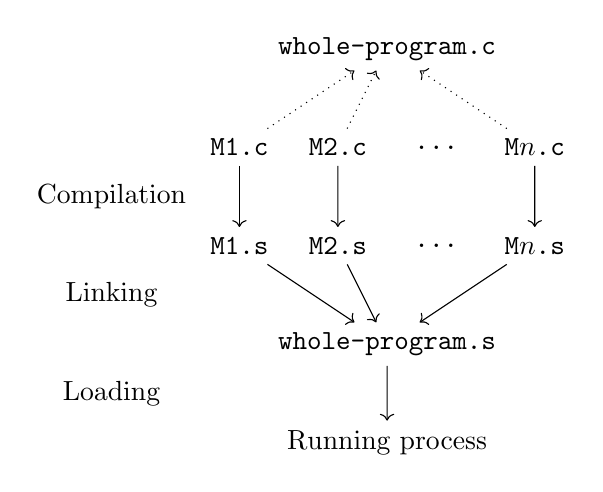
\begin{tikzpicture}[scale=1.25]
        \node (Mb) at (1.5, 0) {Running process};
        \tt
        \node (Ms) at (1.5, 1) {whole-program.s};
        \node (M1c) at (0, 3) {M1.c};
        \node (M2c) at (1, 3) {M2.c};
        \node (etc) at (2, 3) {\ldots};
        \node (Mnc) at (3, 3) {M$n$.c};
        \node (M1s) at (0, 2) {M1.s};
        \node (M2s) at (1, 2) {M2.s};
        \node (ets) at (2, 2) {\ldots};
        \node (Mns) at (3, 2) {M$n$.s};
        \draw (M1c) edge[->] (M1s);
        \draw (M2c) edge[->] (M2s);
        \draw (Mnc) edge[->] (Mns);
        \draw (M1s) edge[->] (Ms);
        \draw (M2s) edge[->] (Ms);
        \draw (Mns) edge[->] (Ms);
        \draw (Ms) edge[->] (Mb);
        \rm
        \node at (-1.3, 2.5) {Compilation};
        \node at (-1.3, 1.5) {Linking};
        \node at (-1.3, 0.5) {Loading};
        \tt
        \node (Mc) at (1.5, 4) {whole-program.c};
        \draw (M1c) edge[->,dotted] (Mc);
        \draw (M2c) edge[->,dotted] (Mc);
        \draw (Mnc) edge[->,dotted] (Mc);
    \end{tikzpicture}
    \caption{CompCert's approximation of the C toolchain}
    \label{fig:process}
\end{figure}
%}}}

Since CompCert is a compiler from C to assembly,
but does not include an assembler or linker,
the model used for verification accounts for
some of these aspects in ithe simplified way
depicted in Fig.~\ref{fig:process}.
The lowest-level objects considered
are CompCert \kw{Asm} programs.
The operation of the linker is approximated by
merging programs, seen as sets of global definitions.
Hence the compilation, linking and execution
of a program composed of the translation units
\texttt{M1.c}, \texttt{M2.c}, \ldots \texttt{M$n$.c},
is modeled by:
\[
    L_\kw{tgt} :=
    \kw{Asm}[C(\texttt{M1.c}) +
             C(\texttt{M2.c}) +
             \cdots +
             C(\texttt{M$n$.c})] \,,
\]
where $C$ is the CompCert compiler,
$+$ denotes CompCert's linking operator for \kw{Asm} programs, and
$\kw{Asm[-]}$ maps an assembly program to its semantics,
in terms of the kind of labelled transition system
defined in \S\ref{sec:sem:closed}.
Note that the loading process is encoded
as part of the definition of the $\kw{Asm}[-]$ language semantics,
which involves the construction of a global environment
laying out the program's code and static data
into the runtime address space,
and performing the usual invocation of a C program's
\kw{main} function.

To formulate compiler correctness,
we must also specify the expected behavior of the target program
in terms of the semantics of the source program.
To this end,
CompCert defines a linking operator
and a whole-program semantics $\kw{Clight}(-)$
for source programs as well,%
\footnote{
  Although CompCert features a frontend for a richer version
  of the C language,
  the simplified intermediate dialect \kw{Clight}
  is usually used as the source language
  when using CompCert to build certified artifacts.
  In particular it is the target language of the
  \texttt{clightgen} utility which
  produces Coq code for a C program's AST,
  which the user can the prove to be correct
  wither manually or with tools such as the VST program logic
  \cite{vst}.
}
allowing the desired behavior to be specified as:
\[
    L_\kw{src} :=
    \kw{Clight}[\texttt{M1.c} + \texttt{M2.c} + \cdots + \texttt{Mn.c}] \,,
\]
and the correctness of CompCert
as a separate compiler
to be stated as $L_\kw{src} \sqsubseteq L_\kw{tgt}$.

%}}}

\subsection{Closed Semantics} \label{sec:sem:closed} %{{{

The language semantics in CompCert are
given as labelled transition systems (LTS).
They model the initial invocation of the \kw{main()} function
and describe a program's behavior in terms of
sequences of observable events.
An event $e \in \mathbb{E}$ denotes an interaction between
the program and its environment;
possible events include system call invocations
and accesses to volatile variables.

Schematically, a CompCert LTS
is a tuple
$L = \langle S, I, {\rightarrow}, F \rangle$
consisting of
a set of states $S$,
a subset $I \subseteq S$ of initial states,
a labeled transition relation
${\rightarrow} \subseteq S \times \mathbb{E}^* \times S$,
and a set
$F \subseteq S \times \kw{int}$
of final states associated with integer results.
A transition $s \stackrel{t}{\rightarrow} s'$
indicates that the state $s$ may transition to state $s'$
through an interaction recorded as the event trace $t \in \mathbb{E}^*$.
The possible behaviors of CompCert LTS fall into four categories:
\begin{itemize}
\item An execution reaching a final state exhibits
    \emph{terminating} behavior.
    For example,
    the following execution generates
    the event trace $t_1 t_2 \cdots t_{n-1}$
    and terminates with exit status $r$:
    \[
        I \ni s_1 \stackrel{t_1}{\rightarrow}
          s_2 \stackrel{t_2}{\rightarrow}
          \cdots \stackrel{t_{n-1}}{\rightarrow}
          s_n \mathrel{F} r \,.
    \]
\item An execution reaching
    an infinite sequence of silent transitions
    is said to be \emph{silently diverging}.
    The following execution silently diverges after
    generating the event trace $t_1 t_2 \cdots t_{n-1}$:
    \[
        I \ni s_1 \stackrel{t_1}{\rightarrow}
          s_2 \stackrel{t_2}{\rightarrow}
          \cdots \stackrel{t_{n-1}}{\rightarrow}
          s_n \stackrel{\epsilon}{\rightarrow}
          s_{n+1} \stackrel{\epsilon}{\rightarrow}
          \cdots
    \]
\item By contrast,
    infinite executions which keep interacting
    are said to exhibit \emph{reactive} behavior.
    The following execution
    exhibits reactive behavior if and only if
    $\forall i \, \exists j \,.\, i \le j \wedge t_j \ne \epsilon$:
    \[
        I \ni s_1 \stackrel{t_1}{\rightarrow}
          s_2 \stackrel{t_2}{\rightarrow}
          s_3 \stackrel{t_3}{\rightarrow}
          \cdots
    \]
\item Finally, an execution which reaches a stuck state
    is said to \emph{go wrong}. It will have the shape:
    \[
        I \ni s_1 \stackrel{t_1}{\rightarrow}
          s_2 \stackrel{t_2}{\rightarrow}
          \cdots \stackrel{t_{n-1}}{\rightarrow}
          s_n \,,
    \]
    where there is no $t, s'$ such that
    $s_n \stackrel{t}{\rightarrow} s'$.
    This is interpreted as an \emph{undefined behavior}:
    it can be refined by any behavior
    admitting $t_1 t_2 \cdots t_{n-1}$ as a prefix.
\end{itemize}

The model outlined above
makes no attempt to model interactions across components,
and is only ever used to
describe the behavior of whole programs.
This makes it challenging to reason about
the behavior of individual compilation units,
although there have been successful attempts in this direction
\cite{sepcompcert,gilhurslatest}.
In any case,
the compiler's correctness property
as described in \S\ref{sec:sem:intro}
only considers uses which follow
the pattern approximated in Fig.~\ref{fig:process}.

To formulate a more fine-grained and flexible
version of the correctness theorem of CompCert,
we need an account of
the behavior of individual translation units.
The model presented in \S\ref{sec:sem:open}
achives this by recoding control transfers
to and from the modeled system explicitly.
These control transfer will need to expose more information
about the internal structure of program states;
in the following section we review the design of
CompCert's memory model,
which all program states are constructed from.

%}}}

\subsection{The CompCert Memory Model} \label{sec:sem:mm} %{{{

The CompCert memory model \cite{compcertmmv2}
is the core algebraic structure
which underlies the semantics of CompCert's languages.
Some of its operations
are shown in Fig.~\ref{fig:mm}.
The idealized version presented here
involves
the type of memory states \kw{mem},
the types of pointers \kw{ptr} and address ranges \kw{ptrrange}, and
the type of runtime values \kw{val}.
To keep our exposition concise and clear,
we will gloss over the technical details
associated with the encoding of offsets
as concrete binary integers,
and the associated modular arithmetic and overflow constraints.

The memory is organized into a finite number of \emph{blocks}.
Each memory block has a unique identifier ($b : \kw{block}$)
represented as a positive integer,
and is equipped with its own independent linear address space.
Block identifiers and offsets are often manipulated together,
as a pair $p = (b, o) : \kw{ptr} = \kw{block} \times \mathbb{Z}$.
New blocks are created by the primitive $\kw{Mem.alloc}$,
with prescribed boundaries for their usable offsets.

A runtime value ($v : \kw{val}$) can be stored at
a given address using the primitive \kw{Mem.store},
and retreived using the primitive \kw{Mem.load}.
Values can be integers (\kw{Vint}, \kw{Vlong}) and
floating point numbers (\kw{Vfloat}, \kw{Vsingle})
of different sizes,
as well as pointers (\kw{Vptr}).
The special value \kw{Vundef}
represents an undefined value;
the simulation relations used by CompCert
usually allow $\kw{Vundef}$
to be refined into a more concrete value.
We will write the refinement relation on values as:
\[
    {\sqsubseteq} := \{(\kw{Vundef}, v), (v, v) \mid v \in \kw{val}\}
\]

The memory model is shared by all of the languages in CompCert.
The states used to define their semantics consist of
a memory component $m : \kw{mem}$,
together with language-specific components
containing additional run-time values ($\kw{val}$).
For higher-level languages,
the language-specific component may consist of
a control stack with local environments for each activation;
for lower-level languages,
the additional component will mainly contain
the values stored in various registers.

\begin{figure} % fig:mm (The CompCert memory model) {{{
  %\footnotesize
  \begin{gather*}
        v : \kw{val} ::= 
          \kw{Vundef} \alt
          \kw{Vint}(n) \alt
          \kw{Vlong}(n) \alt \\
         \qquad \kw{Vfloat}(x) \alt
          \kw{Vsingle}(x) \alt
          \kw{Vptr}(b, o)
    \\
    (b, o) : \kw{ptr} :=
      \kw{block} \times \mathbb{Z}
    \\
    (b, l, h) : \kw{ptrrange} :=
      \kw{block} \times \mathbb{Z} \times \mathbb{Z}
  \end{gather*}
  \begin{align*}
    \kw{Mem.alloc} &:
      \kw{mem} \rightarrow \mathbb{Z} \rightarrow \mathbb{Z} \rightarrow
      \kw{mem} \times \kw{block}
    \\
    \kw{Mem.free} &:
      \kw{mem} \rightarrow
      \kw{ptrrange} \rightarrow
      \kw{option}(\kw{mem})
    \\
    \kw{Mem.load} &:
      \kw{mem} \rightarrow \kw{ptr} \rightarrow \kw{option}(\kw{val})
    \\
    \kw{Mem.store} &:
      \kw{mem} \rightarrow \kw{ptr} \rightarrow \kw{val} \rightarrow \kw{option}(\kw{mem})
    \\
    \kw{Mem.perm} &:
      \kw{mem} \rightarrow \kw{ptr} \rightarrow \mathcal{P}(\kw{perm})
  \end{align*}
  \caption{Outline of the CompCert memory model}
  \label{fig:mm}
\end{figure}
%}}}

%}}}

[XXX: somewhere else]
To compute this behavior
language semantics must rely on a parameter $\chi$
which give the semantics of the runtime functions
relied on by the compiler,
as well as any other library functions
invoked by the user program.
Language semantics must also model
the way in which C programs are loaded
and their \kw{main} function is invoked.

\subsection{Language Interfaces} \label{sec:sem:li} %{{{

The memory model also plays a central role
when describing interactions between program components.
In CompCert languages,
the memory state captures all global state.
Therefore,
under a game-theoretic approach to component semantics,
short of modelling memory accesses explicitly as moves,
the memory state must be passed back-and-forth
alongside all control transfers.

\begin{table}[t] % tbl:li Language interfaces {{{
  \begin{tabular}{clll}
    \hline
    Name & Question & Answer & Description \\
    \hline
    $\mathcal{C}$ & $f[\kw{sg}](\vec{v})@m$ & $v'@m'$ &
      C calls \\
    $\mathcal{L}$ & $f[\kw{sg}](\kw{ls})@m$ & $\kw{ls}'@m'$ &
      Abstract locations \\
    $\mathcal{M}$ & $f(\kw{sp},\kw{ra},\kw{rs})@m$ & $\kw{rs}'@m'$ &
      Machine registers \\
    $\mathcal{A}$ & $\kw{rs}@m$ & $\kw{rs}'@m'$ &
      Arch-specific \\
    $\mathbf{1}$ & n/a & n/a &
      Empty interface \\
    $\mathcal{W}$ & * & $r$ &
      Whole-program \\
    \hline
  \end{tabular}
%  \begin{gather*}
%      \kw{sg} : \kw{signature} ; \:
%      m : \kw{mem} ; \: v : \kw{val} ; \: \vec{v} : \kw{val}^* \\
%      \kw{ls} : \kw{loc} \rightarrow \kw{val} ; \:
%      \kw{rs} : \kw{reg} \rightarrow \kw{val} ; \:
%      \kw{sp}, \kw{ra} : \kw{val}
%  \end{gather*}
  \caption{Language interfaces used in CompCertO}
  \label{tbl:li}
\end{table}
%}}}

More specifically,
our models of cross-module interactions in CompCert languages
are shown in Table~\ref{tbl:li}.
We call each one a \emph{language interface}.
Questions correspond to function invocations,
whereas answers return control to the caller.
Formally,
a language interface is defined as follows.

\begin{definition}
A \emph{language interface} is a tuple
$A = \langle M_A^\kw{Q}, M_A^\kw{A} \rangle$, where
$M_A^\kw{Q}$ is a set of \emph{questions} and
$M_A^\kw{A}$ is a set of \emph{answers}.
\end{definition}

At the source level (language interface $\mathcal{C}$),
questions consist of
the address of the function being invoked
($f : \kw{val}$)
as well as its signature
($\kw{sg} : \kw{signature}$),
the values of its arguments
($\vec{v} : \kw{val}^*$),
and the state of the memory at the point of entry
($m : \kw{mem}$);
answers
consist of the function's return value
and the state of the memory at the point of exit.
In these terms,
a Clight component describes a strategy for the game
$\mathcal{C} \rightarrow \mathcal{C}$.
The component is activated by an incoming $\mathcal{C}$ question
in the right-hand side $\mathcal{C}$ game,
and eventually expected to produce a $\mathcal{C}$ answer.
Conversely,
it may perform external calls by
asking questions in the left-hand side $\mathcal{C}$ game,
which will be answered by the environment.

This language interface is used for Clight and
for the majority of CompCert's intermediate languages,
including the RTL language which is used to perform
most of the compiler's optimizations.
As the backend moves towards lower-level languages,
this is reflected in the language interfaces used:
function arguments are first mapped into
abstract locations alongside local temporary variables
($\mathcal{L}$, used by the LTL and Linear languages).
These locations are eventually split between
in-memory stack slots and a fixed number of machine registers
($\mathcal{M}$, used by the Mach language).
Finally, the target assembly language Asm
consolidates the stack pointer, program counter,
and return address into their own machine registers,
which is reflected in its interface $\mathcal{A}$.

The interface of whole-program execution
can also be described in this setting:
the language interface $\mathbf{1}$ contains no move;
the interface $\mathcal{W}$ has a single trivial question $*$,
and the answers $r \in \kw{int}$
give the exit status of a process.
Hence the original CompCert semantics described in
\S\ref{sec:sem:closed}
can be seen as defining strategies for the game
$\mathbf{1} \rightarrow \mathcal{W}$:
the process can only be started in a single way,
may not perform external calls,
and indicates an exit status upon termination.

%}}}

\subsection{Open Semantics} \label{sec:sem:open} %{{{

Having described the control transfer interfaces
used in the languages of CompCert,
we show how the closed semantics
described in \S\ref{sec:sem:closed}
is generalized in CompCertO
to account for cross-component interactions.

\begin{definition}
Given an \emph{incoming} language interface $B$
and an \emph{outgoing} language interface $A$,
an \emph{labeled transition system for the game $A \rightarrow B$}
is a tuple $L = \langle S, \rightarrow, I, X, Y, F \rangle$.
The relation
${\rightarrow} \subseteq S \times \mathbb{E}^* \times S$ is
a \emph{transition relation} on the set of states $S$.
The handling of incoming calls is specified by
$I \subseteq M_B^\kw{Q} \times S$, which
assigns to each question of $B$ a set of \emph{initial states}, and by
$F \subseteq S \times M_B^\kw{A}$,
which designates \emph{final states} together with corresponding answers.
External calls are specified by
$X \subseteq S \times M_A^\kw{Q}$,
which identifies \emph{interacting states} together with
a corresponding question of $A$ directed to the environment, and
$Y \subseteq S \times M_A^\kw{A} \times S$,
which is used to select a \emph{resumption state}
based on the outcome of the external call
after the environment returns.
We write $L : A \rightarrow B$ to indicate that
$L$ is a labeled transition system for $A \rightarrow B$.
\end{definition}

The interpretation of the generalized LTS described above
follows the one given in \S\ref{sec:sem:closed},
with interactions over the game $A$
as a new source of observable actions.
The main reason for treating
events $e \in \mathbb{E}$ and
interactions $qr \in M_A^\kw{Q} \times M_A^\kw{A}$
differently is that
while events are expected to be the same
between the source and target programs,
the form of interactions varies significantly
and a correpondance between source and target interactions
must be defined explicitly.

%For a small-step semantics
%$L = \langle S, {\rightarrow}, I, X, Y, F \rangle : \kw{semantics}(A,B)$,
%we recognize those states using the predicate:
%\[
%    \kw{stuck}_L(s) :=
%      ({\rightarrow}(s) = \varnothing) \wedge
%      (X(s) = \varnothing) \wedge
%      (F(s) = \varnothing)
%\]
%Taking this into account,
%the immediate behavior of a state $s \in S$
%can be expressed as the interactive computation
%$\kw{step}_L(s) : \mathcal{I}_{M_A^\kw{Q},M_A^\kw{A}}(S)$
%defined as follows:
%\[
%  \kw{step}_L(s) :=
%    \begin{cases}
%      \top & \mbox{if } \kw{stuck}(s) \\
%      {\rightarrow}(s) \sqcup
%      (X(s) \bind \mathbf{I} \bind Y(s)) & \mbox{otherwise,}
%   \end{cases}
%\]
%The overall external behavior of $L$
%can then be given as
%$
%    \llbracket L \rrbracket :
%      M_B^\kw{Q} \rightarrow \mathcal{I}_{M_A^\kw{Q},M_A^\kw{A}}(M_B^\kw{A})
%$
%defined by:
%%Then $\llbracket L \rrbracket$ can be defined as:
%\begin{align*}
%  \llbracket L \rrbracket (q) :=
%    \begin{cases}
%       \top & \mbox{if } I(q) = \varnothing \\
%       I(q) \bind \kw{step}^\infty \bind F & \mbox{otherwise.}
%     \end{cases}
%\end{align*}

%}}}

\subsection{Language Semantics} %{{{

[Give example definitions for Clight and/or Asm here?]

%}}}

\subsection{Simulation Conventions} \label{sec:sem:simconv} %{{{

To establish the correctness of the compiler
at the level of open components,
we will need to relate the behavior of the source component
$p_1$,
expressed as a transition system
$\kw{Clight}(p_1) : \mathcal{C} \rightarrow \mathcal{C}$,
and the behavior of the target program $p_2$,
expressed as
$\kw{Asm}(p_2) : \mathcal{A} \rightarrow \mathcal{A}$.
Since the interactions of these two LTS
are expressed in terms of different language interfaces,
they can only be compared once a correspondance between
C and assembly calls has been defined.
This is the role of simulation conventions.

\begin{definition} % Simulation convention %{{{
A \emph{simulation convention} between the elementary games
$A_1 = \langle M_{A_1}^\kw{Q}, M_{A_1}^\kw{A} \rangle$ and
$A_2 = \langle M_{A_2}^\kw{Q}, M_{A_2}^\kw{A} \rangle$
is as a tuple $\mathbb{R} = \langle W, R^\kw{Q}, R^\kw{A} \rangle$
with $R^\kw{Q} \in \mathcal{R}_W(M_{A_1}^\kw{Q}, M_{A_2}^\kw{Q})$
and $R^\kw{A} \in \mathcal{R}_W(M_{A_1}^\kw{A}, M_{A_2}^\kw{A})$.
We will write $\mathbb{R} : A_1 \Leftrightarrow A_2$.
\end{definition}
%}}}

The set of worlds $W$ is used to
make sure that questions on one hand,
and answers on the other hand,
are related consistently.
For instance,
in CompCertO's overall simulation convention
$\mathbb{C} : \mathcal{C} \Leftrightarrow \mathcal{A}$,
the registers used to store a function's return value
may depend on the signature $\kw{sg}$ used for the call.
As another example,
when an injection pass makes an external call,
we need to make sure the call's final memory states
are related by the same memory injection that was used
for the initial states (or a successor, see \S\ref{sec:corr:inj}).

%}}}

\subsection{Simulations} \label{sec:sem:simconv} %{{{
\label{sec:modsem:ref}

The correctness of CompCert is established in terms of
\emph{backward simulations}%
\footnote{In this usage, \emph{backward} pertains to
  the compilation process,
  rather than the execution of programs.}
between the small-step semantics of the source and target programs,
which are then shown to be sound with respect to trace containement.
In this section,
we define these notions in our updated context.

A backward simulation asserts that any transition in the target program
has a corresponding transition sequence in the source program.
The source transition sequence may be empty,
but to ensure the preservation of silent divergence
this can only happen for finitely many consecutive target transitions.
This is enforced by indexing the simulation relation
over a well-founded order,
and requiring the index to decrease
whenever an empty source transition sequence is used.

A simulation between the small-step semantics
$L_1 : A_1 \rightarrow B_1$ and
$L_2 : A_2 \rightarrow B_2$ will
operate in the context of the refinement conventions
$\mathbb{C}_A : A_1 \Leftrightarrow A_2$ and
$\mathbb{C}_B : B_1 \Leftrightarrow B_2$.
When relating sets of states,
we will want to make sure that
each \emph{target} state has a corresponding \emph{source} state,
but the source program may allow additional behaviors
that are not realized in the target program.
However, to take into account the convention that
empty sets of states correspond to undefined behaviors,
when the source set is empty,
no restrictions are placed on the target state.

\begin{definition}[Backward simulation between sets of states]
We say that $R : \mathcal{R}(S_1, S_2)$ is a
\emph{backward simulation relation
  between the sets $Q_1 \subseteq S_1$ and  $Q_2 \subseteq S_2$}
if the following conditions hold:
\begin{enumerate}
\item
  If $Q_1$ is non-empty,
  then $Q_2$ is non-empty as well.
\item
  If $Q_1$ is non-empty,
  then for all $s_2 \in Q_2$,
  there exists $s_1 \in Q_1$
  such that $(s_1, s_2) \in R$.
\end{enumerate}
We will write $Q_1 \ge_R Q_2$.
\end{definition}

A state $s$ \emph{goes wrong}
if it is neither an interaction nor a final state,
and if there is no transition $s \stackrel{t}{\rightarrow} s'$;
a state $s$ is \emph{safe}
if no state that goes wrong is reachable from $s$
by the relation $\stackrel{\epsilon}{\rightarrow}$.
Safe states will be denoted using the predicate $\kw{safe}(s)$.
We can now define backward simulations.
[XXX: do forward simulations instead?]

\begin{definition}[Backward simulation]
Given
two simulation conventions
$\mathbb{R}_A : A_1 \Leftrightarrow A_2$ and
$\mathbb{R}_B : B_1 \Leftrightarrow B_2$,
and given
$L_1 : A_1 \rightarrow A_1$ and
$L_2 : B_2 \rightarrow B_2$
two labeled transition systems for the corresponding games,
a \emph{backward simulation} between $L_1$ and $L_2$
consists in a
well-founded relation $(I, <)$
together with a family of relations
$(R_i : \mathcal{R}_{W_B}(S_1, S_2))_{i \in I}$
satisfying the following properties:
\begin{description}
\item[Initial states]
  For all $w_B, q_1, q_2$ such that
  $q_1 \ifr{w_B \Vdash \mathbb{R}_B^\kw{Q}} q_2$,
  the condition $I_1(q_1) \ge_{\exists i . w_B \Vdash R_i} I_2(q_2)$ holds.
\item[Progress]
  For all $w_B, s_1, s_2$ such that $s_1 \ifr{w_B \Vdash R_i} s_2$
  with $s_1$ a safe state,
  $s_2$ does not go wrong.
\item[Simulation]
  For all $w_B, s_1, s_2$ such that $s_1 \ifr{w \Vdash R_i} s_2$
  with $s_1$ a safe state, if $s_2 \stackrel{t}{\rightarrow} s_2'$,
  then there exists $i' \in I$ and $s_1' \in S_1$
  such that $s_1' \ifr{w_B \Vdash R_{i'}} s_2'$ and
  such that 
    $s_1 \stackrel{t}{\rightarrow^+} s_1'$, or
    $s_1 \stackrel{t}{\rightarrow^*} s_1' \:\wedge\: i' < i$.
\item[External calls]
  For all $s_1 \ifr{w_B \Vdash R_i} s_2$
  with $s_1$ a safe state, and
  for any question $m_2 \in M_{A_2}^\kw{Q}$
  such that $s_2 \mathrel{X_2} m_2$,
  there exist $w_A \in W_A$ and a question $m_1 \in M_{A_1}^\kw{Q}$
  such that $m_1 \ifr{w_A \Vdash \mathbb{R}_A^\kw{Q}} m_2$.
  In addition, for a corresponding pair of related answers
  $n_1 \ifr{w_A \Vdash \mathbb{R}_A^\kw{A}} n_2$,
  the condition $Y_1(s_1, n_1) \ge_{\exists i . w_A \Vdash R_i} Y_2(s_2, n_2)$ holds.
\item[Final states]
  For all $s_1 \ifr{w_B \Vdash R_i} s_2$
  with $s_1$ a safe state, and
  for any answer $r_2 \in M_{B_2}^\kw{A}$
  such that $s_2 \mathrel{F_2} r_2$,
  there exists a state $s_1'$ silently reachable from $s_1$ and
  an answer $r_1 \in M_{B_1}^\kw{A}$ such that
  $s_1' \mathrel{F_1} r_1$ and $r_1 \ifr{w_B \Vdash \mathbb{R}_B^\kw{A}} r_2$.
\end{description}
We will write $L_1 \ge_{\mathbb{R}_A \rightarrow \mathbb{R}_B} L_2$.
\end{definition}

%}}}

\subsection{Horizontal Composition} \label{sec:sem:linker} %{{{

XXX: the definition of horizontal composition involves
the domains of components,
which so far I haven't addressed in the semantics model.

The interaction of a set of components
can be modelled by the following operator.

\begin{figure} % fig:hcomp {{{
    \begin{gather*}
        \AxiomC{$q \in \kw{dom}(L_i)$}
        \AxiomC{$q \mathrel{I_i} s$}
        \BinaryInfC{$q \mathrel{I} [(i, s) :: \kw{nil}]$}
        \DisplayProof
        \\[1ex]
        \AxiomC{$s \stackrel{t}{\rightarrow}_i s'$}
        \UnaryInfC{$
            [(i, s) :: k]
            \stackrel{t}{\rightarrow}
            [(i, s') :: k]$}
        \DisplayProof
        \\[1ex]
        \AxiomC{$s \mathrel{X_i} q$}
        \AxiomC{$q \in \kw{dom}(L_j)$}
        \AxiomC{$q \mathrel{I_j} s'$}
        \TrinaryInfC{$
            [(i, s) :: k]
            \stackrel{\epsilon}{\rightarrow}
            [(j, s') :: (i, s) :: k]$}
        \DisplayProof
        \\[1ex]
        \AxiomC{$s' \mathrel{F_j} r$}
        \AxiomC{$(s, r, s'') \in Y_i$}
        \BinaryInfC{$
            [(j, s') :: (i, s) :: k]
            \stackrel{\epsilon}{\rightarrow}
            [(i, s'') :: k]$}
        \DisplayProof
        \\[1ex]
        \AxiomC{$s \mathrel{X_i} q$}
        \AxiomC{$\forall j \,.\, q \notin \kw{dom}(L_j)$}
        \BinaryInfC{$[(i, s) :: k] \mathrel{X} q$}
        \DisplayProof
        \\[1ex]
        \AxiomC{$(s, r, s') \in Y_i$}
        \UnaryInfC{$([(i, s) :: k], r, [(i, s') :: k]) \in Y$}
        \DisplayProof
        \\[1ex]
        \AxiomC{$s \mathrel{F_i} r$}
        \UnaryInfC{$[(i, s) :: \kw{nil}] \mathrel{F} r$}
        \DisplayProof
    \end{gather*}
    \caption{Horizontal composition of open semantics}
    \label{fig:hcomp}
\end{figure}
%}}}

\begin{definition}[Horizontal composition] \label{def:hcomp} %{{{
For a language interface $A$
and two transition systems $L_1, L_2 : A \rightarrow A$
with
$L_i = \langle S_i, {\rightarrow}_i, I_i, X_i, Y_i, F_i \rangle$,
the \emph{horizontal composition} of $L_1$ and $L_2$
is defined by:
\begin{align*}
    L_1 \oplus L_2 &:= \langle S^*, {\rightarrow}, I, X, Y, F \rangle \\
    S &:= \sum_{i \in I} S_i
\end{align*}
where the components $\rightarrow$, $I$, $X$, $Y$, $F$
are defined inductively by 
the rules showen in Fig.~\ref{fig:hcomp}.
\end{definition}
%}}}

The horizontal composition operator
allows us to describe the semantics of a
multi-component program
as the composition of the semantics
of its individual components.
In particular,
since we are interested in using CompCertO
to establish the correctness of assembly programs,
the following theorem showing the correctness
of assembly linking is particularly critical.

\begin{theorem} \label{thm:asmlinking} %{{{
For \kw{Asm} programs,
linking is a correct implementation of
semantic composition:
\[
    \forall p_1 p_2 \,.\,
      \kw{Asm}(p_1 + p_2) \le_\kw{id}
      \kw{Asm}(p_1) \oplus \kw{Asm}(p_2)
\]
\begin{proof}
See \texttt{x86/AsmLinking.v} in the Coq development.
\end{proof}
\end{theorem}
%}}}

Once the semantics of the \kw{Asm} program we wish to verify
has been separated into its constituent components,
we can verify each one independently.
This is enabled by the following property,
namely the preservation of simulation by
horizontal composition.

\begin{theorem} \label{thm:simlinking} %{{{
For a simulation convention
$\mathbb{R} : A_1 \Leftrightarrow A_2$
and transition systems
$L_1, L_1' : A_1 \rightarrow A_1$ and
$L_2, L_2' : A_2 \rightarrow A_2$,
the following propery holds:
\[
    \AxiomC{$L_1 \le_{\mathbb{R} \rightarrow \mathbb{R}} L_2$}
    \AxiomC{$L_1' \le_{\mathbb{R} \rightarrow \mathbb{R}} L_2'$}
    \BinaryInfC{$L_1 \oplus L_1' \le_{\mathbb{R} \rightarrow \mathbb{R}} L_2 \oplus L_2'$}
    \DisplayProof
\]
\begin{proof}
See \texttt{common/SmallstepLinking.v}
in the Coq development,
specifically \texttt{compose\_simulation}.
\end{proof}
\end{theorem}
%}}}

This property allows the behavior of a composite semantics
$L_1 \oplus L_2 \oplus \cdots \oplus L_n$
to be refined component by component.

%}}}

\subsection{Loaders} \label{sec:sem:loader} %{{{

XXX: Here, could describe how loaders for various language
interfaces can be defined.
Loaders turn an open semantics such as
$L : \mathcal{C} \rightarrow \mathcal{C}$
into a closed whole-program semantics of type
$\kw{load}(L) : \mathbf{1} \rightarrow \mathcal{W}$.

Problem: the definitions of loaders involve
program skeletons and symbol tables,
which so far I have left out of the semantic model.

%}}}

%}}}

\section{Compiler passes} \label{sec:passes} %{{{

\begin{table*} % tbl:passes Passes of CompCertO %{{{
  \begin{tabular}{lllp{.55\textwidth}}
    \hline
    Language/Pass & Outgoing & Incoming & Description \\
    \hline
    \textbf{Clight} & $\mathcal{C}$ & $\mathcal{C}$ &
      A simpler version of CompCert C \\
    \emph{Thm.~\ref{thm:lprops}} & $(\kw{ext} + \kw{injp})^*$ & $(\kw{ext} + \kw{injp})^*$ & \\
    \kw{SimplLocals} & $\kw{injp}$ & $\kw{inj}$ &
      Pull non-adressable local variables out of memory \\
    \kw{Cshmgen} & \kw{id} & \kw{id} &
      Simplify control structures and type-dependent computations \\
    \hline
    \textbf{Csharpminor} & $\mathcal{C}$ & $\mathcal{C}$ &
      Low-level structured language \\
    \kw{Cminorgen} & $\kw{injp}$ & $\kw{inj}$ &
      Stack allocation of local variables whose address is taken \\
    \hline
    \textbf{Cminor} & $\mathcal{C}$ & $\mathcal{C}$ &
      Low-level structured language; stack allocation of locals \\
    \kw{Selection} & $\kw{ext}$ & $\kw{ext}$ &
      Recognition of operators and addressing modes \\
    \hline
    \textbf{Cminorsel} & $\mathcal{C}$ & $\mathcal{C}$ &
      Like Cminor, with machine-specific operators \\
    \kw{RTLgen} & $\kw{ext}$ & $\kw{ext}$ &
      Construction of the CFG, 3-address code generation \\
    \hline
    \textbf{RTL} & $\mathcal{C}$ & $\mathcal{C}$ &
      Register transfer language \\
    \kw{Tailcall} & $\kw{ext}$ & $\kw{ext}$ &
      Recognition of tail calls \\
    \st{Inlining} & $\kw{injp}$ & $\kw{inj}$ &
      Function inlining \\
    \kw{Renumber} & $\kw{id}$ & $\kw{id}$ &
      Postorder renumbering of the CFG \\
    \st{Constprop} & $\kw{ext}$ & $\kw{ext}$ &
      Constant propagation \\
    \st{CSE} & $\kw{ext}$ & $\kw{ext}$ &
      Common subexpression elimination \\
    \st{Deadcode} & $\kw{ext}$ & $\kw{ext}$ &
      Redundancy elimination \\
    \st{Unusedglob} & $\kw{injp}$ & $\kw{inj}$ &
      Removal of unused static globals \\
    \emph{Thm.~\ref{thm:lprops}} & $\kw{inj}$ & $\kw{inj}$ & \\
    \kw{Allocation} & \kw{alloc} & \kw{alloc} &
      Register allocation \\
    \hline
    \textbf{LTL} & $\mathcal{L}$ & $\mathcal{L}$ &
      Location transfer language \\
    \kw{Tunneling} & $\kw{ext}$ & $\kw{ext}$ &
      Branch tunneling \\
    \kw{Linearize} & \kw{id} & \kw{id} &
      Linearization of the CFG \\
    \hline
    \textbf{Linear} & $\mathcal{L}$ & $\mathcal{L}$ &
      Like LTL, but the CFG is replaced by a linear list of instructions \\
    \kw{CleanupLabels} & \kw{id} & \kw{id} &
      Removal of unreferenced labels \\
    \kw{Debugvar} & \kw{id} & \kw{id} &
      Synthesis of debugging information \\
    \kw{Stacking} & \kw{stacking} & \kw{stacking} &
      Laying out the activation records \\
    \hline
    \textbf{Mach} & $\mathcal{M}$ & $\mathcal{M}$ &
      Like Linear, with a more concrete view of the activation record \\
    \kw{Asmgen} & \kw{asmgen} & \kw{asmgen} &
      Emission of assembly code \\
    \hline
    \textbf{Asm} & $\mathcal{A}$ & $\mathcal{A}$ &
      Assembly language for x86 machines \\
    \hline
  \end{tabular}
  \caption}}

We have explained how the semantic model of CompCert
can be generalized to account for cross-component interaction,
and accordingly defined the semantic model used by CompCertO.
In this section,
we describe how the simulation proofs of
the various passes of CompCert
can be adapted to fit this model.
Owing to the flexibility of our typed relational model,
this adaptation is much easier than
in previous work such as Compositional CompCert.

The passes of CompCertO are summarized in Table~\ref{tbl:passes}.
They are grouped by their source language.
All but the last pass listed under a given language
use it as their target language as well;
the last pass uses the next language as its target.

Each pass is assigned an incoming and outgoing simulation convention,
which is largely determined by the simulation relation
used in the corresponding proof.
For passes whose source and target languages
used the same language interface,
this is determined in particular by the way memory states are related.
For the \kw{Alloc}, \kw{Stacking} and \kw{Asmgen} passes,
we construct more specific simulation conventions
which express the correspondance between
the higher-level and lower-level representations
of function calls and returns.

%\subsection{Overview} %{{{
%
%[Drop/redistribute this?]
%
%The passes of CompCert fall into three categories
%depending on how
%the memory states of their source and target languages are related
%by their correctness proofs:
%\begin{itemize}
%\item \emph{Equality} is used when the memory states
%  in the source and target execution remain identical,
%  for instance when the differences between
%  the source and target programs are mostly a matter of syntax,
%  but they execute in the same way.
%\item \emph{Memory extensions} are somewhat less constrained:
%  the target memory is allowed to contain values that are
%  \emph{more defined} than that of the source memory,
%  and to have less restrictive permissions,
%  so that all operations succeeding on the source memory
%  will succeed on the target memory as well.
%  However,
%  the two memory states must share the same overall structure.
%\item \emph{Memory injection} relations
%  allow the structures of the source and target memories
%  to differ, as specified by an injection mapping
%  (see Example~\ref{ex:meminj}).
%\end{itemize}
%
%Table~\ref{tbl:passes} shows
%the intermediate languages and compilation passes
%used in our version of CompCert,
%together with the respective
%language interfaces and
%simulation conventions
%that are used for each one.
%In the remainder of this section,
%we will explain how these simulation conventions are constructed
%and how the compiler's overall incoming and outgoing conventions
%can be reconciled.
%
%%}}}

\subsection{Identity passes} \label{sec:pass:id} %{{{

The simplest passes of CompCert
use a simulation relation which
restricts the source and target
memory states and values to be identical.
For the passes \kw{Cshmgen}, \kw{Renumber}, \kw{Linearize},
\kw{CleanupLabels} and \kw{Debugvar},
we can use the identity simulation convention
defined below.

\begin{definition}
The \emph{identity simulation convention} for
a language interface $A$ is:
\[
    \kw{id}_A : A \Leftrightarrow A := \langle \{*\}, {=}, {=} \rangle \,.
\]
We abbreviate it as $\kw{id}$ when $A$ can be deduced
from context.
\end{definition}

The simulation proofs for these passes
require very few changes.
The simulation properties for
the interaction and resumption predicates
added to our extended model
can be proved in a single line of proof script.
In fact,
because of various simplifications we perform
to the overall CompCert theories
regarding the management of symbol tables and global environments,
the overall proof size for these passes slightly \emph{decreases}.

%}}}

\subsection{Extension passes} %{{{

For passes where strict equality is too restrictive,
but where the source and target programs
use identical memory layouts,
CompCert uses the \emph{memory extension} relation.
Memory extension allows the values
stored in the target memory state to refine
the corresponding values stored in the source memory;
the target memory state can also
provide more permissions than the source memory,
and in particular blocks may be allocated with
a broader range of addresses in the target memory
than in the source.

We write $\subseteq$ for the memory extension relation.
The relation can be extended to questions and answers,
so that for example $\mathcal{C}$ extension passes
conform to the simulation convention defined as:
\[
    \kw{ext}_\mathcal{C} :=
        \langle \{*\}, {\subseteq}, {\subseteq} \rangle
        : \mathcal{C} \Leftrightarrow \mathcal{C} \,,
\]
where the $\subseteq$ relations on $\mathcal{C}$
moves are defined by the rules:
\begin{gather*}
    \AxiomC{$\vec{v}_1 \mathrel{\vec{\sqsubseteq}} \vec{v}_2$}
    \AxiomC{$m_1 \subseteq m_2$}
    \BinaryInfC{$f[sg](\vec{v}_1)@m_1 \subseteq f[sg](\vec{v}_2)@m_2$}
    \DisplayProof
    \\[1ex]
    \AxiomC{$v_1' \sqsubseteq v_2'$}
    \AxiomC{$m_1' \subseteq m_2'$}
    \BinaryInfC{$v_1'@m_1' \subseteq v_2'@m_2'$}
    \DisplayProof
\end{gather*}
The simulation convention $\kw{ext}_\mathcal{L}$
used by the $\kw{Tunneling}$ proof
is defined in a similar way.

Extension passes are not much more difficult to update
than identity passes.
In particular,
at external calls the exsiting proofs
only require the environment to maintain the extension relation
on memory states.

%}}}

\subsection{Injection passes} %{{{

Although more flexible than equality,
extensions are insufficient
for passes which alter the block structure of the memory.
For these passes,
CompCert uses \emph{memory injections}.
As discussed in the context of Ex.~\ref{ex:meminj},
injection relations $\hookrightarrow$
are parametrized by an \emph{injection mapping}
of type
$\kw{meminj} :=
\kw{block} \rightharpoonup \kw{block} \times \mathbb{Z}$,
which specifies a correspondance between
the addresses of the source and target memory.
The injection relation on values
modifies the refinement relation
by requiring that all pointers be transformed
according the the injection mapping.
The injection relation on memory states
requires that corresponding addresses
hold related values.

Injection passes are more complex than
identity and extension passes,
because ...

[Figure explaining the changes at external calls]

%}}}

\subsection{The \kw{Allocation} pass} %{{{

The \kw{Alloc} pass from \kw{RTL} to \kw{LTL}
uses a memory extension,
but in addition
it is the first pass to modify the external interface of function calls.

\kw{LTL} includes a notion of \emph{abstract locations},
meant to represent the eventual stack slots and machine registers
used at the assembly level.
The values of abstract locations are stored in a \emph{location map},
which complements the memory state and is likewise
is passed across components through
the questions and answers of the language interface $\mathcal{L}$.

Up to \kw{RTL},
arguments are passed as standalone values,
but in \kw{LTL}
they are mapped to abstract locations
depending on the function's signature.
The compiler also expects the values of
locations designated as \emph{callee-save}
to be preserved by function calls.
This is codified in the $\kw{alloc}$
simulation convention, defined as follows:
\begin{gather*}
  \kw{alloc} := \langle
      \kw{signature} \times \kw{locmap}, \:
      R_\kw{alloc}^\kw{Q}, \:
      R_\kw{alloc}^\kw{A} \rangle
  \\[1ex]
  \AxiomC{$\vec{v} \mathrel{\vec{\sqsubseteq}} \kw{args}(sg, ls)$}
  \AxiomC{$m_1 \sqsubseteq m_2$}
  \BinaryInfC{$
      (sg, rs) \Vdash
      f[sg](\vec{v})@m_1
      \mathrel{R_\kw{alloc}^\kw{Q}}
      f[sg](ls)@m_2$}
  \DisplayProof
  \\[1ex]
  \AxiomC{$v' \sqsubseteq \kw{retval}(sg, ls')$}
  \AxiomC{$ls \equiv_\kw{CS} ls'$}
  \AxiomC{$m_1' \sqsubseteq m_2'$}
  \TrinaryInfC{$
      (sg, ls) \Vdash
      v'@m_1'
      \mathrel{R_\kw{alloc}^\kw{A}}
      ls'@m_2'$}
  \DisplayProof
\end{gather*}
where $\kw{args}(sg, ls)$ extracts the values of arguments
stored in the location map $ls$ given a function call signature $sg$,
$\kw{retval}(sg, ls)$ likewise extracts the
values returned by the function call, and
$\equiv_\kw{CS}$ relates location maps whose contents agree
on callee-save locations.

%}}}

\subsection{The \kw{Stacking} pass} %{{{

The \kw{Stacking} pass is the most intricate pass of CompCert,
and a major source of the complexity of related work.

%}}}

\subsection{The \kw{Asmgen} pass} %{{{

\kw{Asm} introduces explicit
program counter, stack pointer and return address registers.
The \kw{Asmgen} pass from \kw{Mach} to \kw{Asm}
uses the following simluation convention:
\begin{gather*}
  \kw{asmgen} := \langle \kw{val} \times \kw{val},
    R_\kw{asmgen}^\kw{Q}, R_\kw{asmgen}^\kw{A} \rangle
  \\[1ex]
  \AxiomC{$\mathit{rs}_1 \uplus
    [\kw{sp} := \mathit{sp}, \kw{ra} := \mathit{ra}, \kw{pc} := f]
    \sqsubseteq \mathit{rs}_2$}
  \AxiomC{$m_1 \sqsubseteq m_2$}
  \BinaryInfC{
    $(\mathit{sp}, \mathit{ra}) \Vdash
     f(\mathit{sp}, \mathit{ra}, \mathit{rs}_1)@m_1
     \mathrel{R_\kw{asmgen}^\kw{Q}}
     \mathit{rs}_2@m_2$}
  \DisplayProof
  \\[1ex]
  \AxiomC{$
    \mathit{rs}_1' \uplus [\kw{sp} := \mathit{sp}, \kw{pc} := \mathit{ra}]
    \sqsubseteq \mathit{rs}_2'$}
  \AxiomC{$m_1' \sqsubseteq m_2'$}
  \BinaryInfC{$
    (\mathit{sp}, \mathit{ra}) \Vdash \mathit{rs}_1'@m_1'
    \mathrel{R_\kw{asmgen}^\kw{A}}
    \mathit{rs}_2'@m_2'$}
  \DisplayProof
\end{gather*}

This concludes our summary of the passes of CompCertO
and the conventions we have been able to use
to characterize their simulation proofs.

%}}}

%}}}

\section{Simulation Algebra} \label{sec:simalg} %{{{

We have described in \S\ref{sec:passes}
the passes of CompCertO
and the types of their simulation proofs.
In this section,
we show how they can be combined to establish
a satisfactory simulation theorem
for the whole compiler.

%\[
%  \begin{array}{cc}
%    \AxiomC{$L \le_{\kw{id}_A \rightarrow \kw{id}_B} L$}
%    \DisplayProof
%    &
%    \AxiomC{$L^\sharp \le_{\mathbb{R}_A \rightarrow \mathbb{R}_B} L^\natural$}
%    \AxiomC{$L^\natural \le_{\mathbb{S}_A \rightarrow \mathbb{S}_B} L^\flat$}
%    \BinaryInfC{$
%      L^\sharp \le_{\mathbb{R}_A \cdot \mathbb{S}_A \rightarrow
%                    \mathbb{R}_B \cdot \mathbb{S}_B} L^\flat$}
%    \DisplayProof
%    \\
%    \AxiomC{$L_1 \le_{\mathbb{R} \rightarrow \mathbf{0}} L_2$}
%    \DisplayProof
%    &
%    \math
%

\subsection{Convention Refinement} %{{{

The core of our simulation algebra is
a notion of refinement for simulation conventions.
The refinement relation $\mathbb{R} \sqsubseteq \mathbb{S}$
captures the idea that the convention $\mathbb{R}$
is more general than the convention $\mathbb{S}$,
so that any simulation accepting $\mathbb{R}$ as its
incoming convention will accept $\mathbb{S}$ as well.

\begin{definition}[Simulation convention refinement] %{{{
Given two simulation conventions
$\mathbb{R}, \mathbb{S} : A^\natural \Leftrightarrow A^\sharp$,
we say that
$\mathbb{R}$ refines $\mathbb{S}$ and write
$\mathbb{R} \sqsubseteq \mathbb{S}$
when the following holds:
\[
    \begin{array}{r@{}c@{\:\Rightarrow\:}c@{}c@{}l}
      \forall w \,.\, m_1 \, m_2 \,.\, &
      m_1 \ifr{w \Vdash R^\kw{Q}} m_2 &
      \exists \, v \,.\, &
      m_1 \ifr{v \Vdash S^\kw{Q}} m_2 &
      \: \wedge \\
      \forall \, n_1 \, n_2 \,.\, &
      n_1 \ifr{v \Vdash S^\kw{A}} n_2 &
      &
      n_1 \ifr{w \Vdash R^\kw{A}} n_2 & \,.
    \end{array}
\]
We write $\mathbb{R} \equiv \mathbb{S}$ when both
$\mathbb{R} \sqsubseteq \mathbb{S}$ and
$\mathbb{S} \sqsubseteq \mathbb{R}$.
\end{definition}
%}}}

The following theorem states the relationship between
simulation convention refinement and forward simulations.

\begin{theorem} %{{{
For
$\mathbb{R}' \sqsubseteq \mathbb{R} : A_1 \Leftrightarrow A_2$ and
$\mathbb{S} \sqsubseteq \mathbb{S}' : B_1 \Leftrightarrow B_2$,
the following holds for all
$L_1 : A_1 \rightarrow B_1$ and $L_2 : A_2 \rightarrow B_2$:
\[
      L_1 \le_{\mathbb{R} \rightarrow \mathbb{S}} L_2 \Rightarrow
      L_1 \le_{\mathbb{R}' \rightarrow \mathbb{S}'} L_2 \,.
\]
\begin{proof}
See \texttt{open\_fsim\_ccref} in \texttt{CallconvAlgebra.v}.
\end{proof}
\end{theorem}
%}}}

%}}}

\subsection{Composing passes} %{{{

The most basic way to combine simulation proofs
is notion of vertical composition outlined below.

\begin{definition}[Composition of simulation conventions] %{{{
Given the language interfaces $A^\sharp, A^\natural, A^\flat$
and the simulation conventions
$\mathbb{R} : A^\sharp \Leftrightarrow A^\natural$ and
$\mathbb{S} : A^\natural \Leftrightarrow A^\flat$,
the composite simulation convention
$\mathbb{R} \cdot \mathbb{S} : A^\sharp \Leftrightarrow A^\flat$ is defined as:
\[
    \mathbb{R} \cdot \mathbb{S} :=
      \langle
        W_R \times W_S, \:
        R^\kw{Q} \cdot S^\kw{Q}, \:
        R^\kw{A} \cdot S^\kw{A}
      \rangle \,.
\]
\end{definition}
%}}}

\begin{theorem}[Composition of simulations] \label{thm:simcomp} %{{{
For the transition systems
$L^\sharp : A^\sharp \rightarrow B^\sharp$,
$L^\natural : A^\natural \rightarrow B^\natural$,
$L^\flat : A^\flat \rightarrow B^\flat$,
and the simulation conventions
$\mathbb{R}_A : A^\sharp \Leftrightarrow A^\natural$,
$\mathbb{R}_B : B^\sharp \Leftrightarrow B^\natural$,
$\mathbb{S}_A : A^\natural \Leftrightarrow A^\flat$, and
$\mathbb{S}_B : B^\natural \Leftrightarrow B^\flat$,
the following holds:
\[
  \AxiomC{$L^\sharp \le_{\mathbb{R}_A \rightarrow \mathbb{R}_B} L^\natural$}
  \AxiomC{$L^\natural \le_{\mathbb{S}_A \rightarrow \mathbb{S}_B} L^\flat$}
  \BinaryInfC{
    $L^\sharp \le_{\mathbb{R}_A \cdot \mathbb{S}_A \rightarrow
                   \mathbb{R}_B \cdot \mathbb{S}_B} L^\flat$}
  \DisplayProof
\]
\begin{proof}
\texttt{compose\_open\_fsim} in \texttt{common/Smallstep.v}.
\end{proof}
\end{theorem}
%}}}

\begin{theorem} % assoc, id, monot {{{
For
$\mathbb{R} : A_1 \Leftrightarrow A_2$,
$\mathbb{S} : A_2 \Leftrightarrow A_3$,
$\mathbb{T} : A_3 \Leftrightarrow A_4$,
the following properties hold:
\begin{gather*}
  {\cdot} \ifr{{\sqsubseteq} \times {\sqsubseteq} \rightarrow
               {\sqsubseteq}} {\cdot}
  \\
  (\mathbb{R} \cdot \mathbb{S}) \cdot \mathbb{T} \equiv
    \mathbb{R} \cdot (\mathbb{S} \cdot \mathbb{T})
  \\
  \mathbb{R} \cdot \kw{id} \equiv
  \kw{id} \cdot \mathbb{R} \equiv
  \mathbb{R}
\end{gather*}
\end{theorem}
%}}}

Using the constructions presented so far,
we can define the simulation convention:
\[
    \mathbb{C}^\flat :=
      \kw{alloc} \cdot
      \kw{ext}_\mathcal{L} \cdot
      \kw{stacking} \cdot
      \kw{asmgen} \,,
\]
and compose the passes \kw{Allocation}--\kw{Asmgen}
to get a simulation of type
$\mathbb{C}^\flat \rightarrow \mathbb{C}^\flat$.

%
%Using this theorem,
%we can compose the successive passes of CompCertO
%to obtain a simulation for the overall compiler.
%However,
%the simulation convention used in the resulting theorem
%
%there are two limitations to this approach:
%\begin{itemize}
%\item
%  Because injection passes use different simulation conventions
%  for their incoming and outgoing calls,
%  they break horizontal compositionality in the sense that
%  Thm.~\ref{thm:simlinking} cannot be used
%  on the resulting simulation properties;
%  indeed,
%  the outgoing relationship
%  between the external calls of one component
%  which are established by the simulation theorem
%  cannot be used to satisfy the
%  incoming relationship which the simulation relies on
%  for another component,
%  because these relationships are different.
%  This propagates to the simulation property
%  obtained from composing all of the compiler's passes.
%\item
%  Another issue with the compilers' simulation convention
%  is that it is very specific to the exact sequence of passes
%  used by CompCertO.
%  This means that a slightly different version of the compiler,
%  or even the same version of the compiler used with different
%  optimization passes,
%  would correspond to a different, incompatible
%  correctness property.
%\end{itemize}
%
%We will address these issues by developing a richer
%\emph{simulation convention algebra}
%and relying on the properties
%of \kw{Clight} and \kw{RTL} to reconcile the incoming and outgoing
%conventions injection passes.
%We start with a more in-depth investigation,
%in the next section,
%of the relational structure of CompCert
%and its language semantics.

%}}}

\subsection{CompCertO conventions} %{{{

With composition and refinement,
we can start outlining some of the properties
of the simulation conventions used by the passes of CompCertO.

\begin{theorem} \label{thm:extinj}
The following property holds:
\[
  \kw{ext} \cdot \kw{inj} \equiv
  \kw{inj} \cdot \kw{ext} \equiv
  \kw{inj} \cdot \kw{inj} \equiv
  \kw{inj}
\]
\begin{proof}
\texttt{ext\_inj}, \texttt{inj\_ext}, \texttt{inj\_inj},
found under \texttt{cklr/}.
\end{proof}
\end{theorem}

These properties make it possible to ``condense''
the whole compiler's incoming convention
into $\kw{inj} \cdot \mathbb{C}^\flat$,
but unfortunately the \kw{injp} convention
does not compose with \kw{ext} and itself in the same way.
To obtain a similar effect,
we construct a Kleene algebra on simulation conventions.

%}}}

\subsection{Kleene Algebra} %{{{

\begin{definition} %{{{
Consider $(\mathbb{R}_i)_{i \in I}$
a family of conventions
with
$\mathbb{R}_i = \langle W_i, R_i^\kw{Q}, R_i^\kw{A} \rangle
  : A_1 \Leftrightarrow A_2$
for all $i \in I$.
The least upper bound
can be defined as
$\sum_{i \in I} \mathbb{R}_i := \langle W, R^\kw{Q}, R^\kw{A} \rangle$
where:
\[
  W := \sum_{i \in I} W_i  \qquad
  \begin{array}{l}
  (i, w) \Vdash R^\kw{Q} \: = \: w \Vdash R_i^\kw{Q} \\[1ex]
  (i, w) \Vdash R^\kw{A} \: = \: w \Vdash R_i^\kw{A} \,.
  \end{array}
\]
We will write $\mathbb{R}_1 + \cdots + \mathbb{R}_n$
for the finitary case $\sum_{i=1}^n \mathbb{R}_i$.
Then for $\mathbb{R} : A_1 \Leftrightarrow A_2$,
we define
$\mathbb{R}^* := \sum_{n \in \mathbb{N}} \mathbb{R}^n$,
where:
\[
  \mathbb{R}^0 := \kw{id} \qquad
  \mathbb{R}^{n+1} := \mathbb{R}^n \cdot \mathbb{R} \,.
\]
\end{definition}
%}}}

These constructions allows us to generalize the compiler's
outgoing simulation convention to
$(\kw{ext} + \kw{injp})^* \cdot \mathbb{C}^\flat$.
The following theorem will also be useful.

\begin{theorem}[Addition and Kleene iteration of simulations] \label{thm:simk} %{{{
The following properties hold:
\[
  \AxiomC{$\forall i \,.\,
    L_1 \le_{\mathbb{R} \rightarrow \mathbb{S}_i} L_2$}
  \UnaryInfC{$
    L_1 \le_{\mathbb{R} \rightarrow \sum_i \mathbb{S}_i} L_2$}
  \DisplayProof
  \quad
  \AxiomC{$L \le_{\mathbb{R} \rightarrow \mathbb{S}} L$}
  \UnaryInfC{$L \le_{\mathbb{R}^* \rightarrow \mathbb{S}^*} L$}
  \DisplayProof
\]
\begin{proof}
See \texttt{cc\_star\_fsim} and the preceding definitions
in \texttt{common/CallconvAlgebra.v}.
\end{proof}
\end{theorem}
%}}}

%}}}

\subsection{Language Properties} %{{{

We have simplified both the incoming and outgoing conventions
use by the whole-compiler simulation,
but they remain distinct and incomparable.
To reconcile them,
we will use the following properties
of \kw{Clight} and \kw{RTL}.

\begin{theorem} \label{thm:lprops} %{{{
These simulations hold
for all programs:
\begin{gather*}
\forall \, p \,.\,
  \kw{Clight}(p)
  \le_{(\kw{ext} + \kw{injp})^* \rightarrow (\kw{ext} + \kw{injp})^*}
  \kw{Clight}(p) \\
\forall \, p \,.\,
  \kw{RTL}(p)
  \le_{\kw{inj} \rightarrow \kw{inj}}
  \kw{RTL}(p)
\end{gather*}
\begin{proof}
Use Thm~\ref{thm:simk},
and our demonstration in \S\ref{sec:cklr} that
\kw{Clight} and \kw{RTL} programs self-simulate under
$\kw{ext}$, $\kw{inj}$ and $\kw{injp}$.
\end{proof}
\end{theorem}
%}}}

By introducing these self-simulations
at strategic points in the overall composition of passes
shown in Table~\ref{tbl:passes},
we can finally establish the following correctness theorem.

\begin{theorem}[Compositional Correctness of CompCertO] %{{{
For a \kw{Clight} program $p^\sharp$
and an \kw{Asm} program $p^\flat$ such that
$\kw{CompCert}(p^\sharp) = p^\flat$,
the following simulation holds:
\[
    \kw{Clight}(p^\sharp) \le_{\mathbb{C} \rightarrow \mathbb{C}}
    \kw{Asm}(p^\flat) \,,
\]
where $\mathbb{C}$ is the simulation convention defined as:
\[
    \mathbb{C} := (\kw{ext} + \kw{injp})^* \cdot \kw{inj} \cdot
      \mathbb{C}^\flat
%      \kw{alloc} \cdot
%      \kw{ext}_\mathcal{L} \cdot
%      \kw{stacking} \cdot
%      \kw{asmgen} \,.
\]
\begin{proof}
Use Thm.~\ref{thm:simcomp} to compose
the correctness proofs of the compiler passes and
self-simulations shown in Table~\ref{tbl:passes}.
By properties of the Kleene star,
the outgoing simulation convention of each of the
passes \kw{SimplLocals}--\kw{Unusedglob}
can be folded into $(\kw{ext} + \kw{injp})^*$
to obtain the overall outgoing convention $\mathbb{C}$.
Likewise, by Thm.~\ref{thm:extinj},
their incoming simulation conventions
can be folded into $\kw{inj}$
to obtain the overall incoming convention $\mathbb{C}$.
\end{proof}
\end{theorem}
%%}}}

%}}}

%}}}

\section{CompCert Kripke Logical Relations} \label{sec:cklr} %{{{

Memory extensions and injections
are useful for simulations
because they are specific instances
of logical relations for the CompCert memory model:
they are compatible with memory operations
in the sense that
performing similar operations on related arguments
yields related results.

\subsection{Definition} %{{{

We formalize this idea by defining
a notion of Kripke logical relations over the CompCert memory model,
closed under composition, and which
admits memory extensions and injections as particular instances.
As we will see,
more complex relations can also be defined,
and this will make relational parametricity theorems
particularly useful.

\begin{definition}[CompCert Kripke logical relation] \label{def:cklr} %{{{
Consider a tuple $R = (W, \leadsto, f, R^\kw{mem})$,
where
$\langle W, \leadsto \rangle$ is a Kripke frame,
$f : W \rightarrow \kw{meminj}$
associates an injection mapping to each world, and
$R^\kw{mem} : \mathcal{R}_{W}(\kw{mem})$
is a Kripke relation on memory states.
We introduce the Kripke relations
$R^\kw{ptr} : \mathcal{R}_W(\kw{ptr})$ and
$R^\kw{ptrrange} : \mathcal{R}_W(\kw{ptrrange})$
defined by the rules:
\[
  \AxiomC{$f_w(b) = (b', \delta)$}
  \UnaryInfC{$(b, o) \ifr{w \Vdash R^\kw{ptr}} (b', o + \delta)$}
  \DisplayProof
  \qquad
  \AxiomC{$(b_1, l_1) \ifr{w \Vdash R^\kw{ptr}} (b_2, l_2)$}
  \AxiomC{$h_1 - l_1 = h_2 - l_2$}
  \BinaryInfC{$(b_1, l_1, h_1) \ifr{w \Vdash R^\kw{ptrrange}} (b_2, l_2, h_2)$}
  \DisplayProof
\]
and the Kripke relation
$R^\kw{val} : \mathcal{R}_W(\kw{val})$
defined by the rules:
\begin{gather*}
  \forall \, v : \kw{val} \,.\,
    \kw{Vundef} \ifr{\Vdash R^\kw{val}} v \qquad
  \kw{Vptr} : {}
    [\Vdash R^\kw{ptr} \rightarrow R^\kw{val}] \\
  \kw{Vint}, \kw{Vlong}, \kw{Vfloat}, \kw{Vsingle} :
    [\Vdash {=} \rightarrow R^\kw{val}] \,.
\end{gather*}
We say that $R$ is a \emph{CompCert Kripke logical relation}
if the properties shown in Fig.~\ref{fig:cklr-def} are satisfied.
\end{definition}
%}}}

\begin{figure} % fig:cklr-def (Definition of CKLRs) {{{
  \footnotesize
  \begin{gather*}
    {\leadsto} \mbox{ is reflexive and transitive} \\
    f \ifr{(\leadsto) \rightarrow \kw{inject\_incr}} f
  \end{gather*}
  \begin{align*}
      \kw{Mem.alloc} :
        &\Vdash R^\kw{mem} \rightarrow {=} \rightarrow {=} \rightarrow
        \Diamond (R^\kw{mem} \times R^\kw{block})
      \\
      \kw{Mem.free} :
        &\Vdash R^\kw{mem} \rightarrow R^\kw{ptrrange} \rightarrow
        \kw{option}^\le(\Diamond R^\kw{mem})
      \\
      \kw{Mem.load} :
        &\Vdash R^\kw{mem} \rightarrow R^\kw{ptr} \rightarrow
        \kw{option}^\le(R^\kw{val})
      \\
      \kw{Mem.store} :
        &\Vdash R^\kw{mem} \rightarrow R^\kw{ptr} \rightarrow R^\kw{val} \rightarrow
        \kw{option}^\le(\Diamond R^\kw{mem})
      \\
      \kw{Mem.perm} :
        &\Vdash R^\kw{mem} \rightarrow R^\kw{ptr} \rightarrow {\subseteq}
  \end{align*}
  \caption{Axioms for CKLRs}
  \label{fig:cklr-def}
\end{figure}
%}}}

The $R^\kw{mem}$ component is given direcly.
We expect $R^\kw{ptr}$ to be functional
(each source pointer has at most one corresponding target pointer),
and to satisfy the following shift-invariance property:
\[
  \AxiomC{$(b_1, o_1) \ifr{R^\kw{ptr}_w} (b_2, o_2)$}
  \UnaryInfC{$(b_1, o_1 + \delta) \ifr{R^\kw{ptr}_w} (b_2, o_2 + \delta)$}
  \DisplayProof
\]
Any such relation can be uniquely specified by
an injection mapping such as $f$.
We expect the remaining components to be consistent with $R^\kw{ptr}$
and $\kw{Vundef}$ to act as a bottom element for $R^\kw{val}$.
Definition~\ref{def:cklr} follows from these conditions.

Note that $w \Vdash R^\kw{val}$
is equivalent to $\kw{Val.inject}(f_w)$
as defined in CompCert.
Furthermore, the relational property associated to $f$,
together with the definitions of
derived relations such as $R^\kw{ptr}$ and $R^\kw{val}$,
ensure that these relations are monotonic in $w$.
However,
this is not usually the case for $R^\kw{mem}$.

%}}}

\subsection{Extensions} %{{{

The simplest CompCert KLR corresponds to memory extensions.
It uses a trivial Kripke frame and injection mapping:
\[
  \kw{ext} :=
    \langle \{*\}, \{(*,*)\}, * \mapsto (b \mapsto b), \kw{Mem.extends} \rangle
\]
Note that $\kw{ext}^\kw{val} = \kw{Val.inject}(b \mapsto b)$
is equivalent to $\kw{Val.lessdef}$,
which is the relation on runtime values that
CompCert uses in conjunction with \kw{Mem.extends}.

%}}}

\subsection{Injections} %{{{

In the same vein,
we can reify memory injections as the CompCert KLR:
\[
  \kw{inj} :=
    \langle
      \kw{meminj},
      {\subseteq}, %\kw{inject\_incr},
      f \mapsto f,
      \kw{Mem.inject}
    \rangle
\]
Here the type \kw{meminj} is used directly
as the KLR's worlds.
The accessibility relation $f \subseteq g$
is the inclusion of partial functions,
called $\kw{inject\_incr}$ in CompCert,
which asserts that for all block identifiers $b, b'$ and offsets $\delta$
such that $f(b) = (b', \delta)$,
then $g(b) = (b', \delta)$ as well.

%}}}

\subsection{Footprint Preservation} %{{{

Passes which use a memory injection as part of their simulation relation
expect external calls to preserve that injection.
In addition,
external calls are expected to only modify
the parts of the source and target memories
that are within the injection's footprint:
addresses that are
related by the injection mapping,
and are granted non-empty permissions
in both memory states.

For instance,
in the \kw{Stacking} pass,
the target memory's stack frames
are extended with spilling locations.
These locations are used in the target program
to keep track of temporary values,
which in the source program are kept
in a local environment separate from the memory state.
The spilling locations are not part of
the injection footprint
because they are unallocated in the source memory;
their preservation across external calls
is essential to the correctness of \kw{Stacking}.

This expectation is reasonable because
external calls
should behave uniformly between the source and target executions.
In particular,
an external function acting on the memory state
should not synthesize block identifiers and pointers,
but can only follow pointers passed as arguments
or fetched from the memory itself.
If it were to access a spilling location in this way in the target execution,
the corresponding source pointer would have to be
related to the target pointer by \kw{Val.inject},
and consequently would either be undefined
or invalid (point to a location without permissions),
so that the source program would go wrong.

Because the CKLR framework is rich enough to express
temporal properties such as the preservation of injection footprints,
this argument can be made precise as a \emph{parametricity} property
(\S\ref{sec:compcert:param}).
For now,
we show how to encode this requirement as a CKLR.

\begin{definition}
The components of the CompCert Kripke logical relation:
\[ \kw{injp} :=
  \langle
    W \times \kw{mem} \times \kw{mem},
    \leadsto_\kw{injp}, \pi_1, R_\kw{injp}^\kw{mem}
  \rangle \]
are defined as follows.
For the injection mappings $f, f'$ and
the memory states $m_1, m_2, m_1', m_2'$,
the relation $(f, m_1, m_2) \leadsto_\kw{injp} (f', m_1', m_2')$
holds when the following conditions are satisfied:
\begin{itemize}
\item $f \subseteq f'$, and any new mappings in $f'$
  must be between newly allocated blocks in $m_1'$ and $m_2'$;
\item any blocks of $m_1$ unmapped by $f$
  must remain unchanged in $m_2$;
\item any locations in $m_2$ unrelated by $f$
  to valid locations of $m_1$ must remain unchanged in $m_2'$;
\item within allocated blocks of $m_1$,
  the permissions assigned to any offset may not increase in $m_1'$
  (this helps ensure that $\leadsto_\kw{meminj}$ is transitive).
\end{itemize}
The relation $R_\kw{injp}^\kw{mem}$ is defined by the rule:
\[
  \AxiomC{$m_1 \ifr{f \Vdash \kw{Mem.inject}} m_2$}
  \UnaryInfC{$m_1 \ifr{(f, m_1, m_2) \Vdash R_\kw{injp}^\kw{mem}} m_2$}
  \DisplayProof
\]
\end{definition}

%}}}

\subsection{Relational Parametricity} \label{sec:compcert:param} %{{{

For each language interface
$\mathcal{X} \in \{ \mathcal{C}, \mathcal{L}, \mathcal{M}, \mathcal{A} \}$,
a CKLR
$R = \langle W, {\leadsto}, f, R^\kw{mem} \rangle$ can be promoted to
a simulation convention
$\mathcal{X}[R] : \mathcal{X} \Leftrightarrow \mathcal{X}$.
For example
we define $\mathcal{C}[R] : \mathcal{C} \Leftrightarrow \mathcal{C}$
as follows:
\[
    \mathcal{C}[R] := \langle
      W, \:
      ({=} \times {=} \times {R^\kw{val}}^* \times R^\kw{mem}), \:
      \Diamond (R^\kw{val} \times R^\kw{mem})
    \rangle \,.
\]
Such operators preserve composition
in the sense that $\mathcal{X}[R ; S] = \mathcal{X}[R] \cdot \mathcal{X}[S]$.

Because the semantics of CompCert languages
are expected to be well-behaved with respect to
invariance properties of the memory model,
we can prove for each language of CompCert
a parametricity theorem of the form
$
    \forall R \,.\,
      \llbracket p \rrbracket
        \le_{\mathcal{X}[R] \Rightarrow \mathcal{X}[R]}
      \llbracket p \rrbracket
$.
Since both sides of the relation are identical,
the simulations can be iterated
to obtain similar properties in terms of $\mathcal{X}[R]^*$.

In particular,
we use this approach to establish the following properties,
which will be useful to derive our final correctness theorem:
\begin{gather}
    \forall R \,.\,
      \kw{Clight} \llbracket p \rrbracket
        \le_{\mathcal{C}[R]^* \Rightarrow \mathcal{C}[R]^*}
      \kw{Clight} \llbracket p \rrbracket
      \label{eqn:clight}
      \\
    \forall R \,.\,
      \kw{RTL} \llbracket p \rrbracket
        \le_{\mathcal{C}[R] \Rightarrow \mathcal{C}[R]}
      \kw{RTL} \llbracket p \rrbracket
      \label{eqn:rtl}
\end{gather}
In addition,
the CKLRs defined above satisfy the following
composition properties:
\[
  \mathcal{C}[\kw{inj}] \cdot \mathcal{C}[\kw{inj}] \equiv
  \mathcal{C}[\kw{ext}] \cdot \mathcal{C}[\kw{inj}] \equiv
  \mathcal{C}[\kw{inj}] \cdot \mathcal{C}[\kw{ext}] \equiv
  \mathcal{C}[\kw{inj}] \,.
\]

%}}}

%}}}

\section{Related and Future Work} %{{{

\subsection{Game Semantics} %{{{

Game semantics first came to prominence
in the context of functional programming languages when
it was used to construct
the first fully abstract models for PCF
\cite{pcfajm,pcfho},
building on partial game models for linear logic
\cite{gsll,gsllaj}.
Subsequent work
extended the approach to account for a variety of
language features such as
state \cite{gsia},
control \cite{gscontrol} and
nondeterminism \cite{gsnondet}.
In particular,
while much of this work initially
targeted sequential programming languages,
investigations of concurrent game models
have been particularly fruitful.

More low-level applications of games have also been proposed,
for instance see the work on interface theories
and interface automata \cite{ia,gmos,itcd,gtf},
and games have been used in the context of modal logic
to model properties of open systems
\cite{atl,altref}.

Although in this paper we have only considered a very simple game model,
in the future we hope to draw from the slew of existing game semantics research
to extend the framework of refinement-based game semantics
to a variety of settings,
and in particular to extend our model
to stateful and concurrent strategies.

%}}}

\subsection{Abstraction} %{{{

Although our treatment of abstraction (\S\ref{sec:monad:abs})
remains quite rudimentary,
we hope to develop a more comprehensive understanding
of abstraction in the context of refinement-based game semantics
by exploring connections with existing research,
in particular with
the theory of abstract interpretation \cite{absint,aif}
and its applications to game models \cite{aigp}.

On a more practical side,
\emph{certified abstraction layers} \cite{popl15,osdi16,ccal}
have been proposed as a general verification methodology
and used to prove the correctness of the operating system kernel CertiKOS.
We hope refinement-based game semantics
can eventually be used to generalize
certified abstraction layers to heterogenous settings.

%}}}

\subsection{Monads and Kleene Algebra} %{{{

Monads equipped with
typed Kleene algebra structures
have been studied under the names of
\emph{preordered monads} \cite{pom} and
\emph{Kleene monads} \cite{kleenem},
in the latter case establishing various decidability results.
Although our interaction monad (\S\ref{sec:monad:def})
comes short of constituting a Kleene algebra
(in particular, as in FailKAT \cite{failkat}
the axiom $x \cdot \mathbf{0} = \mathbf{0}$ does not hold),
it may be possible to embed it in a more well-behaved setting
and take advantage of some of these results.
In particular,
Damien Pous' work on Kleene algebra with converse
and extensive library of associated Coq tactics
offer promising opportunities for proof automation.

Interaction trees \cite{itrees}
represent another approach
related to our interaction monad,
formalized in Coq in the context of the DeepSpec project \cite{deepspec}.
Interaction trees
come out of the research on \emph{algebraic effects},
and are constructed as the free monad
for a user-specified effect signature.
Rather than sets of traces,
their representation uses Coq's coinductive types.

%}}}

%\subsection{TODO}
%
%\begin{itemize}
%\item
%  Limitation:
%  we model linking as in CompCompCert,
%  but do not yet verify a form of linking as specified in SepCompCert
%\item
%  Limitation:
%  liveness properties not expressible as refinement
%\item
%  Linear vs branching time,
%  Vardi's argument for trace semantics
%  as the externally observable things
%\end{itemize}

%}}}

\bibliographystyle{abbrv}
\bibliography{lwcc}

\end{document}
